\documentclass[12pt]{book}
\usepackage[utf8]{inputenc}
\usepackage[italian]{babel}
\usepackage{multicol}
\usepackage{listings}
\usepackage{color}
\usepackage{titlepic}
\usepackage{appendix}
\usepackage{float}
\usepackage{csquotes}
\definecolor{dkgreen}{rgb}{0,0.6,0}
\definecolor{gray}{rgb}{0.5,0.5,0.5}
\definecolor{mauve}{rgb}{0.58,0,0.82}

\lstset{frame=none,
  language=Java,
  aboveskip=3mm,
  belowskip=3mm,
  showstringspaces=false,
  columns=flexible,
  basicstyle={\small\ttfamily},
  numbers=none,
  numberstyle=\tiny\color{gray},
  keywordstyle=\color{blue},
  commentstyle=\color{dkgreen},
  stringstyle=\color{mauve},
  breaklines=true,
  breakatwhitespace=true,
  tabsize=3
}

\addto\captionsenglish{\renewcommand{\figurename}{Fig.}}
\usepackage[sorting=none]{biblatex}
\renewbibmacro{in:}{}
\usepackage{graphicx}
\graphicspath{ {./images/} }
\addbibresource{./bib.bib}

\title{
\includegraphics[width=5cm, height=5cm]{images/Stemma_unipi.png}
    \\\textsc{\small Laurea in Informatica (classe L-31)\\Dipartimento di Informatica\\Università di Pisa}\\\vfill Sperimentazione di Chaos testing per il monitoraggio di un’infrastruttura Fog federata}
\date{}

\begin{document}



\begin{titlepage}

\begin{center}
    
\includegraphics[width=5cm, height=5cm]{images/Stemma_unipi.png}
    \\\textsc{Laurea in Informatica (classe L-31)\\Dipartimento di Informatica\\Università di Pisa}
\end{center}

\begingroup
\let\newpage\relax%
\maketitle
\endgroup
\begin{multicols}{3}
\noindent
\\\\\textbf{Relatori:}\\Federica Paganelli\\Antonio Brogi\\Stefano Forti\\ \columnbreak\linebreak \columnbreak\linebreak
\\\\\textbf{Candidato:}\\Francesco Buti
\end{multicols}
\end {titlepage}

\newpage
\renewcommand{\contentsname}{Indice}
\renewcommand{\listfigurename}{Indice delle Figure}
\renewcommand{\listtablename}{Indice delle Tabelle}
\tableofcontents

\newpage
\listoftables
\listoffigures

\chapter{Introduzione}
In questo capitolo sono descritti il contesto (Sezione 1.1) (cloud computing, fog computing, chaos engineering), gli obiettivi e la metodologia della tesi (Sezione 1.2), di cui infine sarà presentata la struttura (Sezione 1.3).
    \section{Contesto}
    Nell'ultimo decennio, il \textit{cloud computing} si è affermato come un modello per consentire l'accesso di rete onnipresente, conveniente e su richiesta a un insieme condiviso di risorse informatiche configurabili (ad esempio, reti, server, archiviazione, applicazioni e servizi), che può essere fornito e rilasciato rapidamente con il minimo sforzo di gestione o interazione con il fornitore di servizi \cite{nistcloud}.Si tratta dunque di un modello che si fonda sulla flessibilità e scalabilità dei sistemi IT, che consente di ottenere una rapidità di implementazione dei servizi cloud stessi e, d’altra parte, maggiori affidabilità e continuità di servizio \cite{treccani}. Proposto per la prima volta nel 2014 \cite{fog} come estensione del paradigma cloud, il Fog Computing è un modello a più livelli che facilita la scalabilità delle risorse di calcolo dal cloud all'\textit{Internet of Things} (IoT). Il Fog facilita l'implementazione di applicazioni e servizi distribuiti, e si compone di nodi fisici o virtuali, residenti tra i dispositivi IoT e i servizi centralizzati Cloud. I nodi fog possono essere organizzati in gruppi verticalmente (per supportare l'isolamento) o orizzontalmente (per supportare la federazione) così da ridurre al minimo il tempo di richiesta-risposta da e verso le applicazioni supportate \cite{nistfog}. Gli ambienti Fog sono caratterizzati da:
    \begin{itemize}
        \item Presenza pervasiva di risorse di calcolo al limitare (\textit{edge}) della rete, location awareness e basse latenze
        \item Elevata distribuzione geografica
        \item Vasta reti di sensori/attuatori
        \item Mobilità dei nodi
        \item Eterogeneità delle risorse e delle tecnologie di comunicazione
        \item Interoperabilità e federazione di infrastrutture
    \end{itemize}
    Nel complesso, il Fog rappresenta al tempo stesso un'estensione e un miglioramento del paradigma Cloud, in supporto ad applicazioni IoT che debbano rispettare precisi parametri di Qualità di Servizio (QoS), in particolare la bassa latenza sulle connessioni \cite{brogi-forti}.
    In questo contesto, FogMon \cite{FogMon} è stato recentemente proposto come soluzione di monitoraggio di infrastrutture in modo non invasivo, che fosse in grado di tollerare cambiamenti e fallimenti dell'infrastruttura monitorata. FogMon è il prototipo di un servizio di monitoraggio distribuito open source, scritto in C++ e in grado di monitorare l'hardware e le risorse virtualizzate su diversi nodi di elaborazione Cloud-IoT, la \emph{QoS} di rete tra tali nodi (in termini di misurazioni di banda e latenza end-to-end), nonché i dispositivi IoT disponibili. Inoltre, è dotato di una topologia di overlay peer-to-peer auto-organizzante con meccanismi di auto-ristrutturazione e aggiornamenti di monitoraggio differenziale, che offrono scalabilità, tolleranza agli errori e basso sovraccarico di comunicazione. Una prima sperimentazione di FogMon è avvenuta su un'infrastruttura di piccola scala (13 nodi) nell'area di Pisa \cite{FogMon}.
    
    
    Per sperimentare e mettere a punto FogMon in ambienti di più larga scala, il gruppo di ricerca ``Service-Oriented, Cloud and Fog Computing" (SOCC) dell'Università di Pisa ha condotto e portato a termine il progetto LiSCIo (\textit{Lightweight Self-Adaptive Cloud and IoT Monitoring across Fed4Fire+ testbeds}), finanziato dal progetto europeo Fed4Fire+ nel programma Horizon 2020 \cite{Horizon}.
    
    Il lavoro oggetto di questa tesi si inserisce nel più ampio contesto di LiSCIo, con l'ambizione di sperimentare tecniche ispirate al Chaos Engineering \cite{gremlinchaos} per contribuire all'obiettivo di LiSCIo di testare e migliorare FogMon. Il Chaos Engineering, infatti, è stato recentemente proposto e utilizzato per testare la capacità di sistemi distribuiti su larga scala di resistere a condizioni ``turbolente", anche in ambiente di produzione. Non a caso, le tecniche di Chaos Engineering sono sempre più usate in ambito Cloud e Fog \cite {princofchaos} e sono sembrate un candidato ideale per contribuire agli esperimenti di LiSCIo.
    \section{Obiettivi e Metodologia}
    L'obiettivo di questa tesi è quello di testare FogMon sfruttando tecniche ispirate al chaos engineering per individuare i suoi eventuali punti di debolezza, in modo da correggerli e migliorare l'affidabilità del prototipo.
    
    
    La tesi è stata suddivisa in tre fasi: 
    \begin{itemize}
        \item La prima parte è stata dedicata alla formazione e ricerca delle basi teoriche preliminari, in particolare è stato effettuato uno studio delle tecniche di chaos engineering e una ricerca degli strumenti adatti per l’adozione di tali tecniche su un’architettura distribuita.
        \item La seconda fase ha previsto la realizzazione di un programma di supporto, in grado di automatizzare i test su un’istanza di Fogmon, dispiegata su una porzione dell'infrastruttuta federata Fed4Fire+ \cite{Fed4Fire+} senza la necessità di intervento manuale per l'esecuzione dei comandi, nè per le fasi di raccolta e di analisi dei dati 
        \item La terza fase prevede la stesura di un piano degli esperimenti, la loro esecuzione e la raccolta dei dati sul comportamento di Fogmon, per trarre conclusioni sul suo funzionamento e suggerire eventuali messe a punto 
    \end{itemize}
    \section{Struttura della Tesi}
    La seguente sezione presenta una sintesi della struttura della presente tesi divisa per capitoli.
    \begin{description}
    \item [Capitolo 2] Il secondo capitolo illustra le conoscenze preliminari. In particolare, la prima parte si focalizza sul sistema oggetto della sperimentazione di Chaos Testing, ossia FogMon, un programma per il monitoraggio delle risorse e delle applicazioni distribuite su nodi in ambiente Fog. La seconda parte di questa sezione presenta le basi teoriche e il concetto di chaos engineering; lo studio delle tecniche qui riportate è stato fondamentale per la ricerca degli strumenti necessari a testare FogMon, oltre all’organizzazione del piano di test. La conclusione di questo capitolo vedrà anche una breve presentazione del testbed (Fed4Fire) che ha fornito le risorse computazionali e di rete necessarie per lo svolgimento degli esperimenti.
    \item [Capitolo 3] Il terzo capitolo evidenzia la progettazione del piano di test e degli obiettivi della sperimentazione, per poi porre l'attenzione sul programma creato per automatizzare gli esperimenti; verrà inoltre presentato il processo di scelta degli strumenti di chaos engineering usati per svolgere la batteria di test su istanze di Fogmon.
    \item [Capitolo 4] Il quarto capitolo termina la descrizione del lavoro svolto con un resoconto dei test effettuati e dei risultati ottenuti. Questi ultimi si sono rivelati utili a migliorare FogMon stesso e a fornire indicazioni su possibli malfunzionamenti.
    \item [Capitolo 5] Nel quinto capitolo, conclusivo, si esamina il percorso svolto durante la tesi, al fine di comparare gli obiettivi raggiunti con quelli inizialmente prefissi; verrà poi svolta una considerazione finale sull’applicabilità delle tecniche viste in altri progetti, con tutti gli eventuali limiti.
    \end{description}
    

\chapter{Conoscenze preliminari}
In questo capitolo descriveremo il funzionamento di FogMon (Sezione 2.1), le basi teoriche del Chaos Engineering (Sezione 2.2) e il progetto a cui fa riferimento il testbed su cui è stato distribuito FogMon in fase di verifica (Sezione 2.3).
    
    
    \section{Fogmon}
    Come menzionato nel Capitolo 1, FogMon è un prototipo, realizzato in C++, per il monitoraggio di infrastrutture Fog, in particolare delle risorse hardware (CPU, memoria, disco rigido), della QoS delle connessioni end to end (latenza, banda) e della presenza di dispositivi IoT nella rete \cite{FogMon}.
    
    
    FogMon può essere dispiegato su qualsiasi topologia di rete TCP/IP (previa configurazione) ed è costituito da due tipologie di componenti distribuite, ovvero i leader e i follower. I follower sono i responsabili delle misurazioni hardware e QoS e vengono assegnati a dei gruppi, ognuno dei quali fa riferimento a un leader. Un esempio di organizzazione di FogMon è illustrato in Figura \ref {fig:fogmon1}.
    
    \begin{figure}
        \begin{center}
            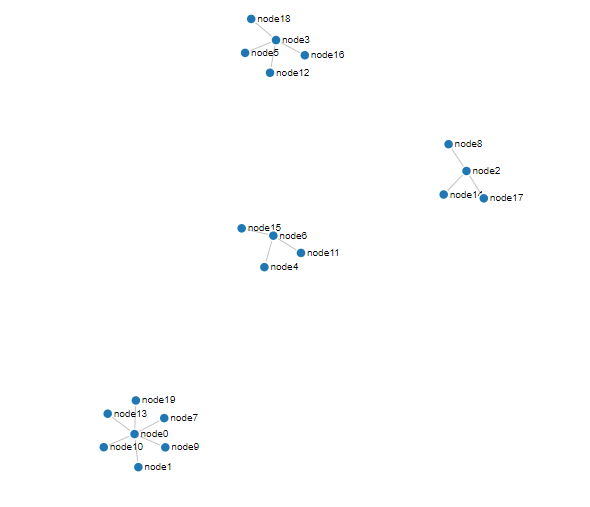
\includegraphics[width=10cm, height=10cm]{images/fogmon.PNG}
            \label {fig:fogmon1}
            \caption {Esempio di organizzazione di FogMon}
        \end{center}
    \end {figure}
    
    
    Attualmente FogMon è rilasciato come immagine Docker \cite{docker}; questo facilita l’installazione e l’esecuzione su qualsiasi macchina in grado di supportare container Docker e di gestire connessioni TCP/IP.
    
    FogMon orchestra diversi tool per raggiungere il suo scopo:
    \begin {itemize}
        \item Hyperic Sigar \cite{sigar} per il monitoraggio hardware e ICMP per la misura della latenza end-to-end (tramite ping)
        \item iperf3 \cite{iperf} ed Assolo \cite{assolo} per ottenere informazioni sulle prestazioni della banda (attivamente con iperf, passivamente con Assolo)
    \end{itemize}
    Leader e follower comunicano tra loro scambiandosi messaggi in formato JSON, sfruttando connessioni TCP. Ogni nodo archivia i dati e le misurazioni in un proprio database SQLite3.
    
    La flessibilità di FogMon risiede anche nella possibilità, per i nodi, di cambiare ruolo (da follower a leader e viceversa) e favorire la costruzione di una topologia migliore e più efficiente, in modo adattivo.
        \subsection{Follower}
        Essendo sviluppato per un ambiente Fog, FogMon assume che i nodi possano rapidamente entrare e uscire dalla rete su cui è distribuito. I follower, pertanto, possono effettuare connessioni e disconnessioni senza che queste operazioni impattino negativamente sul sistema.
        
        
        La topologia di Fogmon viene costruita sulla base di un criterio di prossimità, per cui ogni follower viene assegnato al gruppo del leader verso il quale ha la minima latenza \textit{end-to-end}; quando un nodo si unisce all’ambiente monitorato da FogMon (come follower), conosce inizialmente solo l’indirizzo del leader specificato nella configurazione iniziale. Il nodo a cui si connette il follower agirà da intermediario per fornire la lista degli altri leader a cui il follower potrebbe connettersi.
        
        
        Da qui, il follower eseguirà delle misurazioni della latenza verso ognuno dei leader appena reperiti per connettersi al nodo che presenta il valore più basso, garantendo così il rispetto del criterio di prossimità. i follower cercano sempre il leader con la latenza minore: questo processo di divisione dà origine ai gruppi, ovvero insiemi di follower sotto lo stesso leader. Il processo appena descritto vale anche nel caso in cui un follower non riesca più a raggiungere il proprio leader o nell’eventualità in cui, tramite controlli periodici, un follower individui un leader migliore di quello attuale. 
        
        
        Un altro aspetto importante si identifica nel processo di misurazione della larghezza di banda, eseguito dal nodo Follower, per capirne il livello di affidabilità; FogMon, come accennato, utilizza due sistemi di rilevazione della banda:
        \begin{itemize}
            \item Iperf3, un sistema di rilevazione attiva e, pertanto, intrusiva \cite{iperf}
            
            \item Assolo, un sistema di rilevazione passiva, ma meno affidabile \cite{assolo}
        \end{itemize}
        Per combinare il meglio dei due strumenti, FogMon si ispira al modello ibrido di Marttinen et al. \cite{marttinen}, che riduce a un terzo il numero di misurazioni attive e, pertanto, diminuisce l'intasamento della banda mantenendo comunque dati validi.
        
        Per ridurre ulteriormente il sovraccarico di rete, FogMon invia dati di monitoraggio sia hardware che QoS (uso dela CPU e della memoria, traffico in entrata e uscita, latenza), da follower a leader, basandosi su un sistema di aggiornamenti differenziali. In dettaglio, i follower ripetono la comunicazione di dati comparabili a quelli già misurati e inviati precedentemente, ma solo quelli la cui media o varianza dei valori del report, se confrontata con quelli del report precedente, differisce più di una soglia impostata (ovvero 10\% per impostazione predefinita) dall'ultimo aggiornamento eseguito. Vista la necessità di ridurre lo spazio di archiviazione sfruttato da FogMon, solo le ultime 30 misurazioni vengono conservate nel database di ciascun nodo.\\
        \subsection{Leader}
        FogMon organizza il proprio overlay in modo che il numero dei leader sia pari alla radice del numero totale dei nodi, approssimata all'intero successivo.
        
        
        I nodi leader sono responsabili dell’aggregazione dei dati ricevuti dai follower come risultato del loro monitoraggio. Si occupano inoltre dell’organizzazione della topologia peer-to-peer basandosi sulle metriche misurate dagli altri nodi e sulle informazioni reperite mediante le operazioni di “gossiping” \cite{jelasity}, ovvero lo scambio di dati tra i leader. Ogni leader effettua il monitoraggio del nodo su cui è in esecuzione. I leader raccolgono i dati dai follower che monitorano, i quali riportano periodicamente i dati che misurano.
        
        Infine, ogni leader riesce, tramite la comunicazione con gli altri leader (gossiping), a memorizzare i dati dei follower di altri gruppi.
        
        
        Ad ogni lasso di tempo stabilito, ogni Leader seleziona un altro Leader casuale e invia un report completo sul proprio gruppo di Follower. In aggiunta, il Leader ignora qualsiasi follower che risulti disconnesso, ossia che non ha inviato report negli ultimi due heartbeat. I valori di latenza e banda vengono stimati dai leader \cite{FogMon}, basandosi sull'assunzione che le tecnologie di accesso a Internet (ad esempio, xDSL, 3G, 4G) siano asimmetriche e rappresentino un collo di bottiglia nella comunicazione, specialmente tra i nodi che risiedono ai margini di Internet.
        \subsection{Ricalcolo della topologia}
        FogMon è in grado di decidere autonomamente e adattivamente quali siano i nodi più indicati (in base alle misurazioni di latenza tra i nodi) per agire da leader e come organizzarli in gruppi. Per garantire l'accuratezza delle stime di banda e latenza tra gruppi diversi, FogMon può ristrutturare l'overlay peer-to-peer tra Leader e Follower.
            La ristrutturazione della topologia di rete viene eseguita quando:
            \begin{itemize}
                \item la dimensione della rete raddoppia (o dimezza) rispetto all'ultima ristrutturazione, il che implica che più (o meno) Leader dovrebbero essere designati per gestire la complessità del monitoraggio
                
                \item la qualità del raggruppamento misurata tramite l'indice di Davies-Bouldin \cite{davies-bouldin} (rapporto tra la latenza intergruppo e intragruppo) della topologia corrente supera un parametro soglia, selezionata a 3 per impostazione predefinita.
            \end{itemize}
        Ogni volta che un Leader scopre che una delle due condizioni vale, viene avviata una procedura per il ricalcolo della topologia di FogMon; più leader, anche  contemporaneamente, possono avviare questa procedura.
        
        I leader che ricevono la richiesta, ma non ne hanno iniziata una a loro volta, si limitano a riconoscere il nodo che avvia la procedura; eventuali altri leader che hanno avviato la richiesta, invece, dovranno confrontarsi per trovare il nodo incaricato di gestire il processo di ristrutturazione della topologia.
        
        A questo punto, il leader che guida il ricalcolo invia un messaggio di avvio a tutti gli altri leader, che iniziano a elaborare
        una nuova topologia candidata, sfruttando l'algoritmo k-medoids \cite {k-medoids}. Ogni Leader coinvolto propone una soluzione (e una valutazione sulla qualità di questa soluzione), che verrà candidata come possibile nuova topologia. 
        
        Tutti i nodi che devono cambiare ruolo svolgono questa operazione prima dell'avvio del nuovo overlay della rete; i nuovi leader attendono quindi il termine di tutti cambiamenti di ruolo. I follower, invece, sfruttano le informazioni raccolte durante il ricalcolo della topologia per selezionare il leader più vicino ad essi.
        
        
        \subsection{FogMonEye}
        FogMonEye \cite{FogMonEye} è un microservizio REST sviluppato specificamente per FogMon nell'ambito dell'esperimento LiSCIo \cite{FogMon}. Può essere ospitato su un server esterno, il suo compito primario è quello di collezionare i risultati degli esperimenti effettuati, rendendoli disponibili tramite API REST e un'interfaccia grafica web.
        
        FogMonEye raccoglie i dati che riceve dai nodi leader e li confronta con la topologia impostata inizialmente per configurare l'esperimento. Tale operazione permette di calcolare i seguenti dati: 
        \begin{itemize}
            \item L'errore relativo sulle stime di banda e latenza nei gruppi
        
            \item L'errore relativo sulle stime di banda e latenza tra gruppi
        
            \item Il consumo di risorse in un determinato lasso temporale (uso massimo, minimo e medio di CPU, Memoria e banda)
        
            \item Il tempo necessario per riorganizzare l'overlay di FogMon dopo un cambio dell'infrastruttura, causato da una ristrutturazione della topologia 
            
            \item Una rappresentazione grafica dell'attuale overlay di topologia di FogMon, suddiviso in gruppi 
        \end{itemize}
        I dati appena elencati, ad eccezione dell'ultimo, vengono organizzati in fasi dell'esperimento (dette ``momenti"). La figura \ref{fig:Eye} mostra un esempio di resoconto di un esperimento monitorato da FogMonEye.
        \begin{figure}
        \begin{center}
            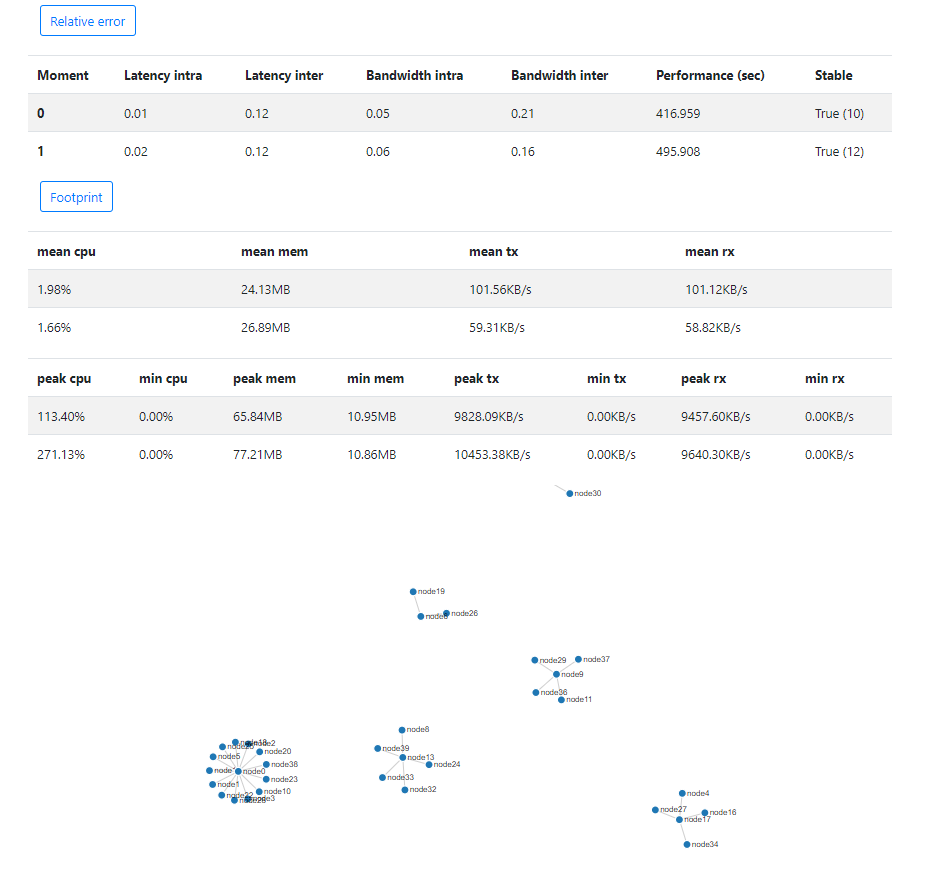
\includegraphics[width=15.6cm, height=13.4cm]{images/Eye.PNG}
            \label {fig:Eye}
            \caption {Esempio di esperimento monitorato da FogMonEye}
        \end{center}
        \end {figure}
        
        
        FogMonEye permette anche di monitorare più esperimenti contemporaneamente e di conservare, al termine, i risultati. Ogni esperimento viene identificato da un ID di sessione, determinato inizialmente tramite l'invio di una specifica a FogMonEye. Per ogni sessione è possibile, inoltre, accedere mediante richieste http a tutti i dati raccolti.
    \newpage
    \section{Chaos Engineering}
    Il Chaos Engineering \cite{princofchaos}\cite{gremlinchaos} è un insieme di tecniche di testing volto a ricercare errori nel sistema mediante l’iniezione volontaria e programmata di fallimenti, in modo da controllare la reazione e possibilmente aumentare la resilienza del sistema di fronte a tali eventi. Questo permette di rivelare comportamenti del programma altrimenti non identificabili, di prevederne le conseguenze sugli utenti e di risolvere tali mancanze il prima possibile.
    
    L'uso del chaos engineering non deve essere sostitutivo delle classiche metodologie di testing, quanto un'integrazione che si rivela particolarmente utile in sistemi che basano il proprio funzionamento su nodi interconnessi \cite{queue}. La caratteristica del testing classico è quella di avere un input e un output già previsti, pertanto non genera alcuna conoscenza completamente nuova su come si comporterà il sistema se dovesse verificarsi un fallimento. Al contrario, con il chaos testing si eseguono esperimenti più ampi, per simulare anomalie infrastrutturali non pianificate. Tutto ciò consente di ottenere nuove conoscenze sui comportamenti, le proprietà e le prestazioni del sistema.
    
   Tra i pionieri del Chaos Engineering troviamo Netflix, che nel 2011 ha proposto Chaos Monkey \cite{Netflix}. Si tratta di uno strumento per testare la resilienza della sua infrastruttura IT. Funziona disabilitando intenzionalmente i server nella rete di produzione di Netflix per testare come i sistemi rimanenti rispondono all'interruzione. L'origine del nome ``Chaos Monkey" è spiegata in \cite{Martinez}:
    
    \emph{``Immagina una scimmia che entra in un `data center', queste `fattorie' di server che ospitano tutte le funzioni critiche delle nostre attività online. La scimmia strappa i cavi in modo casuale, distrugge i dispositivi e getta tutto ciò che trova. La sfida per i responsabili IT è progettare il sistema informativo di cui sono responsabili in modo che possa funzionare nonostante queste scimmie, che nessuno sa mai quando arriveranno e cosa distruggeranno "}.
    
    Dopo Netflix, la necessità di costruire un sistema resiliente e pronto a reagire ai guasti sta spingendo molte altre aziende ad adottare il chaos engineering. Realtà come Amazon \cite{amazon}, Google \cite{Google} e Facebook \cite{Facebook} stanno già adoperando queste tecniche per migliorare i loro sistemi distribuiti, o parti di essi.
    Un altro esempio è da ricercare nella National Australia Bank \cite{NAB}, anch’essa pioniera nello sviluppo di sistemi con l'aiuto del Chaos Engineering. 
    
    
    Il Chaos Engineering può aiutare a identificare errori di disegno di un software distribuito, dovuti a un ampio insieme di assunzioni errate da parte degli sviluppatori \cite{miles}, ad esempio:
    \begin{itemize}
        \item La rete non presenta punti deboli, latenze elevate o problemi di banda
        
        \item La topologia non muta nel tempo
        
        \item I costi di manutenzione e le risorse necessarie alla comunicazione sono identici tra implementazioni diverse 
        
        \item Il sistema è sorvegliato da un amministratore 
        
        \item La potenza di calcolo dei dispositivi non è un problema 
    \end{itemize}
    Tali ipotesi chiaramente non sono da considerare valide nello sviluppo di un’architettura software distribuita, dispiegata su una rete reale, composta da dispositivi fallibili e soggetti a possibili errori di rete.
        \subsection{Esperimento di chaos}Di seguito si riporta il metodo di creazione degli esperimenti di chaos, a partire dalla formulazione dell’ipotesi fino alla sua verifica \cite{miles}\cite{jones} .
        
        Un esperimento di \textit{Chaos Engineering} prevede la creazione di una \textit{Steady State Hypotesis} (ipotesi di stato stabile) e una prima verifica di questa ipotesi per confermare la stabilità del sistema. In seguito, si applica un ``metodo" (fallimento che può compromettere l'ipotesi) e si esegue una seconda verifica della \textit{Steady State Hypotesis}, al fine di identificare, se c'è stata, una deviazione. Possiamo riassumere l'iter appena descritto per un esperimento di \textit{Chaos Engineering} con la figura \ref{fig:5-6miles}.
        \begin {figure}
        \begin{center}
            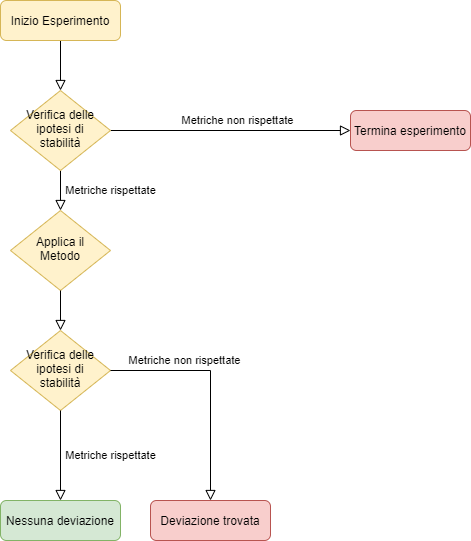
\includegraphics[width=11cm, height=13cm]{images/56miles.png}
            \caption {Passaggi di un esperimento di chaos engineering}
            \label{fig:5-6miles}
        \end{center}
        \end {figure}
        Se al termine della procedura si osserva che l'ipotesi non è rispettata, siamo di fronte a un errore del sistema. In questo caso è necessario ripristinare le condizioni precedenti all'esperimento e implementare una soluzione per evitare che si verifichi nuovamente.
        Nel seguito sono spiegati in dettaglio le fasi di creazione dell'ipotesi e del metodo, di raccolta e di analisi dei dati e di verifica delle ipotesi.
        \subsection{Creazione dell’ipotesi e del ``metodo"}
        È importante, come prima cosa, definire delle metriche per descrivere il funzionamento del sistema, ovvero che alcune assunzioni stabiliscano quale sia il comportamento corretto del software. Parliamo, in questo caso, di \emph{steady state hypotesis}, ossia di ipotesi di funzionamento del sistema in condizioni di stabilità. Secondo \cite{miles}:
        
        
        \emph{``l'ipotesi [dello steady state] esprime, entro determinate tolleranze, ciò che costituisce normale per la parte del sistema testata dall'esperimento di Chaos}.
        
        
        Le ipotesi create definiscono i “limiti” delle azioni che il software dovrebbe poter effettuare e, quindi, modellano quale debba essere il suo funzionamento. Tali ipotesi sono verificabili tramite dei parametri misurabili (ed eventualmente soggetti a una certa tolleranza).
        
        L'applicazione del chaos engineering richiede la verifica di tutte queste ipotesi, per identificare la condizione di stabilità prima e dopo l'iniezione di fallimenti infrastrutturali. Tipicamente le \textit{steady state hypotesis} indicano i comportamenti attesi in merito all’integrità e validità dei dati dell’applicazione, ai tempi delle risposte del sistema all’utente. Prendendo ad esempio Netflix, la società utilizza la velocità con cui i clienti premono il pulsante di riproduzione su un dispositivo di streaming video come parametro, definendo questa metrica come ``flussi al secondo" \cite {cheatsheet}.
        
        
        Il metodo di un esperimento di Chaos definisce le azioni che influenzeranno il sistema e causeranno le condizioni turbolente (ossia il caos) che dovrebbero essere applicate al sistema di destinazione.
        
        
        I fallimenti iniettati quindi non sono, come suggerirebbe il nome “chaos”, casuali. La formulazione di un’ipotesi comporta la ricerca e lo studio di tutti gli scenari che potrebbero portare al fallimento di essa o di altre ipotesi; pertanto, per ogni Steady State Hypotesis verranno realisticamente pensati più metodi per testare più scenari (ad esempio la degradazione della QoS di rete, il crash di un nodo, un errore software).
        
        
        L’iniezione del fallimento deve essere controllabile ed osservabile in modo che la reazione del sistema sia identificabile nel guasto provocato e, pertanto, rimediabile in caso di comportamenti indesiderati. Questa fase deve chiaramente essere effettuata sotto controllo, previo backup del sistema, per evitare che avvengano danni irreversibili al sistema su cui viene eseguito il test, o ai dati del software stesso, e deve essere accompagnata da una strategia di ripristino definita come \textit{rollback} \cite{miles}. Ciò è realizzabile in due tipologie di ambienti:  
        \begin{itemize}
            \item un testbed, dove l'esecuzione del software è puramente a fini di prova e pertanto un eventuale guasto non comporta danni all’infrastruttura o ai dati di un sistema vero e proprio. In questo caso non è necessario un punto di ripristino né una strategia di \textit{rollback}, oppure 
            \item un ambiente di produzione controllato, presumibilmente già più resistente ai fault, con un backup dei dati e misure di sicurezza per l’hardware, accompagnati dalla strategia di rollback per evitare di danneggiare un sistema in funzione.
        \end{itemize}
        Alle due possibilità appena elencate, è possibile affiancare una metodologia CI/CD (continuous integration/continuous delivery) per creare un flusso di integrazione e distribuzione continuo, particolarmente utile nelle fasi di integrazione e test \cite{cicd}.
        \subsection{Analisi dei dati e verifica delle ipotesi}
        La raccolta delle risposte, da automatizzare laddove le metriche di riferimento siano molteplici, deve essere seguita dalla loro analisi. L'analisi consiste principalmente nel verificare tutte le \textit{steady state hypotesis} formulate sul corretto funzionamento del programma. Tale passaggio è importante perchè se si riscontrano deviazioni dalle condizioni attese è stata identificata una potenziale debolezza del sistema.
        
        Come menzionato precedenemente, l'ipotesi dello stato stazionario viene utilizzata due volte: una volta all'inizio dell'esecuzione dell'esperimento e poi di nuovo quando il metodo dell'esperimento ha completato la sua esecuzione:
        \begin{itemize}
            \item All'inizio dell'esecuzione di un esperimento, viene valutata l'ipotesi per decidere se il sistema in oggetto è in uno stato stabile. Se il sistema target si discosta dalle aspettative dell'ipotesi a questo punto, l'esperimento deve essere interrotto, poiché non ha alcun valore dato che il sistema non è riconoscibilmente stabile sin dall'inizio.
            \item Il secondo utilizzo dell'ipotesi dello stato stazionario costituisce il suo ruolo principale nell'esecuzione di un esperimento. Dopo l'applicazione del metodo, la \textit{Steady state hypotesis} viene nuovamente confrontata con il sistema bersaglio. Questo è il punto critico dell'esecuzione di un esperimento, perché rappresenta il momento in cui si possono identificare delle deviazioni, che rischiano di presentarsi nuovamente nel caso in cui il sistema sia sottoposto a condizioni simili a quelle causate dal metodo.
        \end{itemize}
        \paragraph{Chaos Cards}
        In \cite{miles} si descrive come per ogni esperimento sia possibile riassumere le componenti principali in \textit{Chaos Cards}, ovvero un'istanza di \textit{Chaos Experiment} che include:
        \begin{itemize}
            \item La \textit{Steady State Hypotesis}
            \item Le metriche di verifica delle ipotesi (ossia lo spettro di valori accettabili su parametri misurabili)
            \item Il metodo da applicare
            \item Il piano di \textit{Rollback} in caso di deviazione
        \end{itemize}

    \section{Fed4Fire+ e JFed}
    Come accennato nel Capitolo 1, la sperimentazione si è svolta nell'ambito del progetto LiSCIo \cite{FogMon}, il cui scopo è quello di testare e mettere a punto FogMon sfruttando le risorse fornite da Fed4Fire+.
    
    
    Fed4FIRE + è un progetto nell'ambito del programma Horizon 2020 dell'Unione Europea, che offre una federazione di testbed Next Generation Internet (NGI) \cite{Fed4Fire+}.
    
    
    Con le risorse fornite da Fed4Fire+, LiSCIo mira a rendere FogMon in grado di gestire le variazioni nella rete su cui è distribuito, insieme ai possibili fallimenti dei nodi da cui la rete stessa è composta.
    
    
    Fed4Fire+ mette a disposizione vari strumenti per facilitare le sperimentazioni. Tra questi  Jfed \cite{jfed}, un software basato su Java per l'uso di testbed. Tale strumento utilizza un sistema di credenziali e di certificati per autenticare e autorizzare gli utenti su questi testbed. L'utente può creare nuovi esperimenti trascinando da un'area di selezione i tipi di nodi che intende utilizzare.
    
    
    In Figura \ref{fig:jfed} vediamo un esempio di esperimento creato tramite l'interfaccia di Jfed: dopo aver trascinato alcuni nodi, l'utente può selezionare su quale banco di prova desidera eseguire l'esperimento. È possibile eseguire una configurazione aggiuntiva come la selezione di un nodo specifico, la modifica del funzionamento predefinito sistema e selezionare uno script da eseguire all'avvio del nodo. È possibile anche tracciare connessioni di rete tra i nodi; questa operazione causerà la creazione di una VLAN all'interno del testbed prescelto.
    \begin {figure}
    \begin{center}
            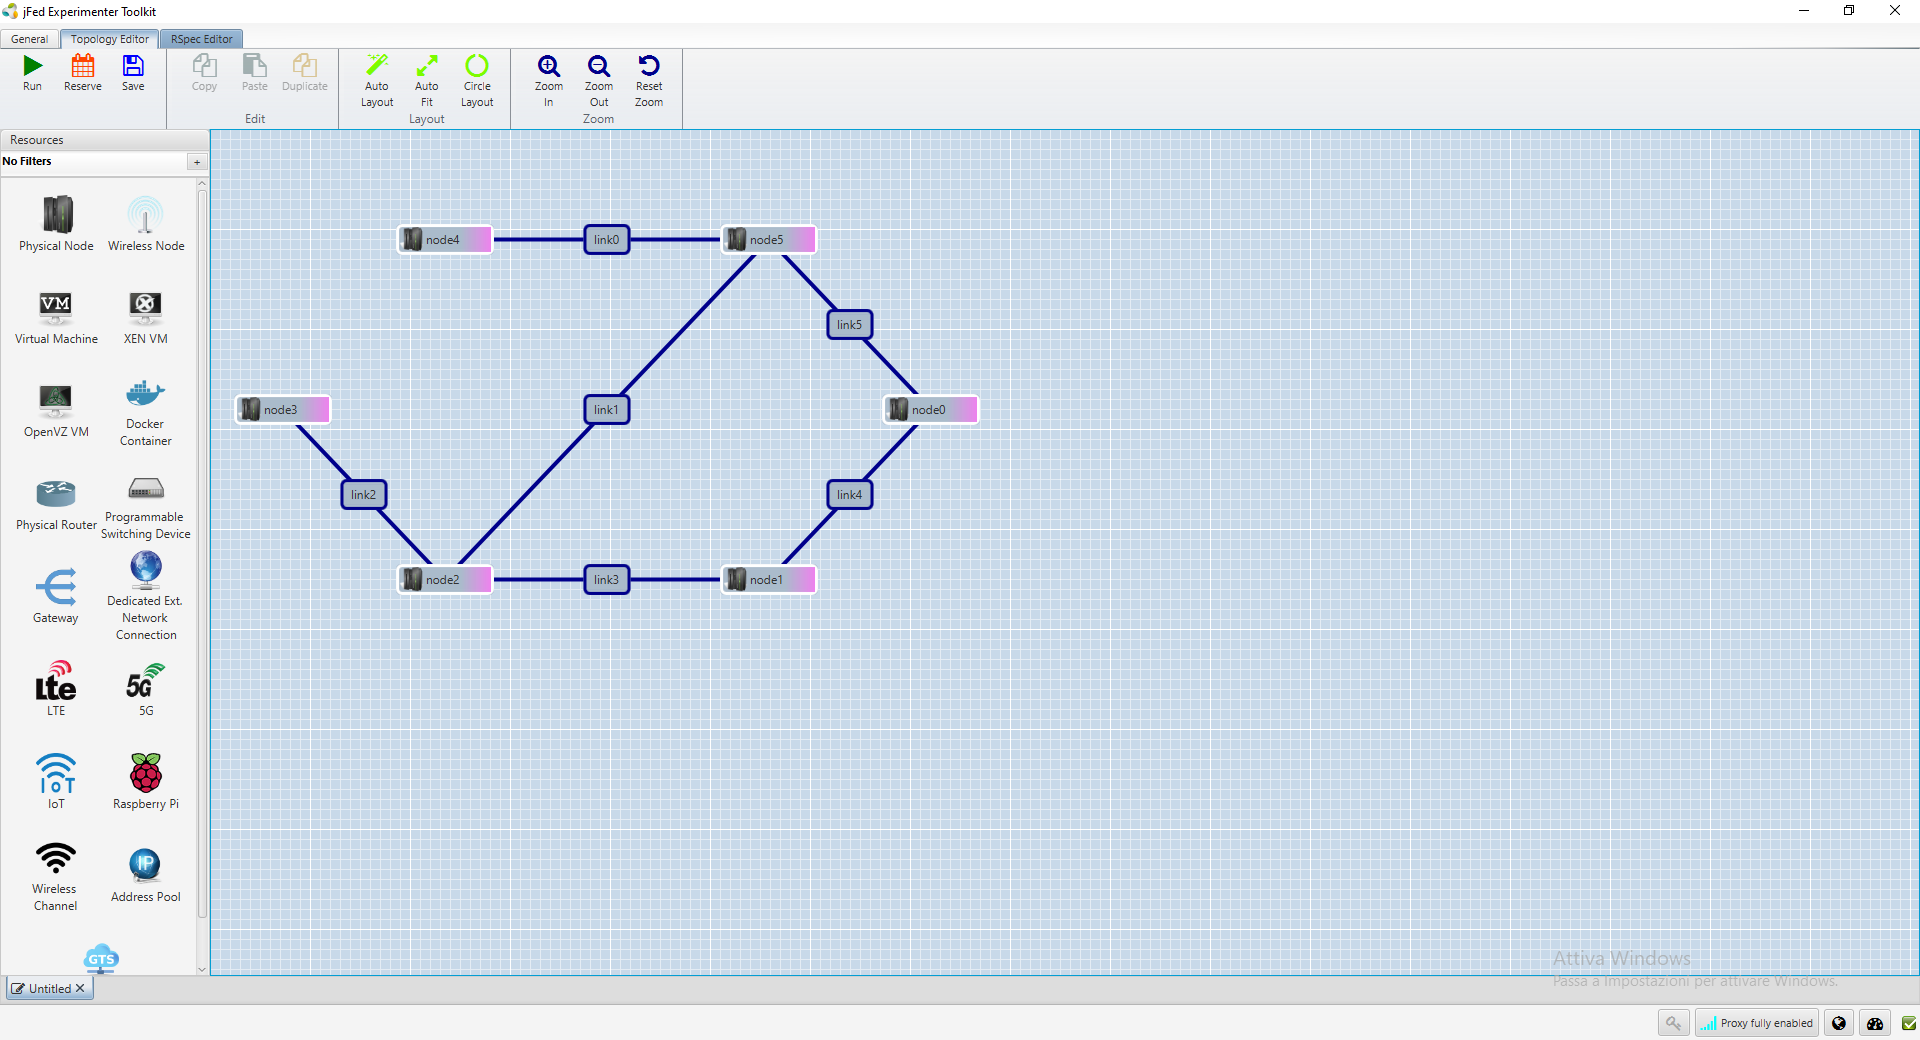
\includegraphics[width=13cm, height=7cm]{images/jfed.png}
            \caption {Esempio di esperimento su jfed}
            \label {fig:jfed}
    \end{center}
    \end {figure}
    
    
    I nodi utilizzati per la sperimentazione sono stati ospitati da:
    \begin{itemize}
        \item Virtual wall \cite {vw}, ospitato e gestito da imec e composto da due datacenter, Virtual Wall 1 (206 nodi) e Virtual Wall 2 (159 nodi). All'interno di LiSCIo i nodi di Virtual Wall sono stati sfruttati per imitare i nodi Cloud di una rete Fog
        \item CityLab \cite {cl}, un testbed destinato alla sperimentazione di reti wireless e 5G. Si trova nel centro della città di Anversa, in Belgio, e appartiene all'Università di Anversa/imec. Il testbed è situato nelle strade dentro e intorno al campus cittadino dell'Università di Anversa, in un'area di circa 0,5 km per 0,5 km. L'hardware attualmente è ospitato in 32 sedi con altre 22 pianificate. Ogni luogo ha il proprio gateway collegato alle case sulla strada o installato su un palo al di sopra di un tetto. Citylab punta sulla sperimentazione in rete per aumentare la maturità della connettività delle \emph{smart cities} \cite {clpdf} e per questo i suoi nodi sono stati usati all'interno di LiSCIo per imitare le risorse edge di una rete Fog.
    \end{itemize}

\chapter{Progettazione e Implementazione dei Chaos Test}
In questo capitolo saranno descritti l'iter seguito per pianificare la sperimentazione, gli obiettivi prefissati al momento della progettazione e l'organizzazione dei test (Sezione 3.1).


Sarà poi esposto il processo di scelta dello strumento di Chaos Engineering usato per l'applicazione dei metodi, in supporto agli esperimenti (Sezione 3.2).

Infine, verrà descritto sinteticamente il programma creato appositamente per automatizzare la sperimentazione (Sezione 3.3).
    \section{Progettazione dei Chaos Test}
    \label{subsec:cards}
    Gli esperimenti condotti hanno seguito il formato delle \textit{Chaos Cards}, sulla base della metodologia descritta nella Sezione 2.2.3 (\textit{Steady State Hypotesis}, Metriche di verifica, metodo, \textit{Rollback}).
    
    L'ambiente della sperimentazione consiste in un'instanza di FogMon dispiegato su un \textit{testbed}, dunque il piano di \textit{Rollback} può essere ignorato a favore di un riavvio del sistema dopo la correzione della deviazione. Questa strategia infatti non comporta danni all'infrastruttura o perdita di dati significativi.
    
    
    Come anticipato nella Sezione 2.2, lo scopo di un esperimento di Chaos Engineering è scoprire le deviazioni inattese nel comportamento di un sistema, per correggerle ed aumentare la sua resilienza. Nel nostro caso, la sperimentazione di FogMon ha l'obiettivo di evidenziare, dove presenti, queste deviazioni e, possibilmente, fornire dati utili per correggerle.
    \subsection{Ipotesi di stabilità, metriche di misura}
    Per identificare le \textit{Steady State Hypotesis} di FogMon è stato svolto un periodo di monitoraggio e di analisi del prototipo. Come risultato dell'osservazione sono state formulate le seguenti ipotesi:
    \begin{itemize}
        \item H1: Il tempo massimo per la configurazione di FogMon, dopo l'avvio del calcolo della topologia, è definito e limitato a un tempo pari a 20 volte il valore del parametro \textit{time-report}, specificato nella configurazione di lancio iniziale di FogMon, con una tolleranza pari al valore di un \textit{time-report}
        \item H2: La qualità del \textit{clustering}, misurata in termini di banda e latenza, si mantiene al di sopra di una soglia prefissata (il calcolo genera un numero intero, sfruttando l'indice di Davies-Bouldin, che deve essere minore di 50)
        \item H3: I cambiamenti di stato e/o delle misure dei nodi di un gruppo, sono noti al leader entro un tempo massimo, dipendente dai parametri della configurazione di lancio iniziale di FogMon
    \end{itemize}
    Ad ognuna di queste \textit{Steady State Hypotesis} sono state affiancate delle metriche di verifica e dei metodi di sperimentazione, che riportiamo in seguito. In Figura \ref{fig:cards} è riportato uno schema di tali ipotesi con le relative metriche e i metodi utilizzati per gli esperimenti.
    \newpage    
    \begin{figure} [H]
        \begin{center}
            \begin{center}
                \begin{tabular}{|c|c|c|c|c|c|c|c|}
                    \hline
                    Steady state & Metriche di & Metodi\\
                    Hypotesis & valutazione & applicati\\
                    \hline
                    & \textbf{M1}: Organizzazione immutata  & \\
                    & per 40 propagation-time &\\
                    &&\\
                    \textbf{H1}: Tempo massimo & \textbf{M2}: Errore nelle misurazioni & Follower failure\\
                    di configurazione & inter/intra-gruppo $\leq$ 25\% & Leader failure\\
                    &&\\
                    & \textbf{M3}: Tempo massimo di &\\
                    & riconfigurazione limitato &\\
                    & dai parametri iniziali &\\
                    \hline
                    & \textbf{M1}: Se nodi = N, & \\
                    & Leader = $\lceil\sqrt{N}\rceil$ & \\
                    &&\\
                    \textbf{H2}:Qualità del & \textbf{M2}: Latenza di ogni Follower & Link failure\\
                    clustering & verso il proprio leader $\leq$ & Follower failure\\
                    & latenza verso altri leader & Leader failure\\
                    &&\\
                    & \textbf{M3}: Indice di qualità $\leq$ &\\
                    & soglia massima &\\
                    \hline
                    & \textbf{M1}: Il database del Leader  & \\
                    & di ogni gruppo elimina  & \\
                    & ogni 10 \textit{propagation-time} & Follower failure\\
                    \textbf{H3}: Diffusione dei & i dati più vecchi di 3 \textit{heartbeat} & Link failure\\
                    cambiamenti nel gruppo & & Stress test\\
                    & \textbf{M2}: L'ultimo report di ogni & \\
                    & Follower deve comparire nel &\\
                    & database del suo Leader &\\
                    &  entro due \textit{heartbeat} &\\
                    \hline
                \end{tabular}
            \end{center}
            \caption {{Le \textit{Chaos Cards} degli esperimenti con FogMon}}
            \label {fig:cards}
        \end{center}
    \end{figure}
    
    \paragraph{Tempo massimo di configurazione} 
    Questa ipotesi (H1) consiste nell'assunzione che, dopo la configurazione iniziale o in seguito all'avvio del processo di riconfigurazione, FogMon raggiunga un grado di stabilità (che definiremo come ``stabilità debole") entro un limite di tempo massimo. Si utilizzano quindi tre metriche per verificarne la validità:
    \begin{itemize}
        \item L'organizzazione dell'overlay di FogMon in Leader e Follower non cambia per 40 periodi consecutivi di comunicazione Leader-Leader (ovvero 40 volte il valore di \textit{propagation-time}, uno dei parametri di configurazione di FogMon)
        \item Tutte le misurazioni della QoS dei collegamenti e dell'hardware sono state eseguite almeno una volta in ciascun gruppo e mostrano un errore inferiore al 25\%.
        \item La riconfigurazione ha un tempo limite calcolato in base al valore di \textit{heartbeat} e di \textit{propagation-time} specificati nella configurazione iniziale di FogMon
    \end{itemize}
    Questa prima ipotesi, se verificata tramite le metriche sopracitate, indica che FogMon si è riconfigurato e ha mantenuto lo stesso overlay per un periodo sufficientemente lungo da essere considerato ``stabile". Dopo questo controllo è sensato verificare le metriche delle altre due ipotesi per capire se FogMon, in questa ``stabilità debole", funziona correttamente.
    
    
    \paragraph{Qualità del clustering} 
    Per questa ipotesi (H2) è necessario definire delle metriche in grado di verificare il rispetto del criterio di prossimità, la corretta valutazione della qualità del \textit{Clustering} e il rapporto numerico Leader-Follower, ovvero:
    \begin{itemize}
        \item I leader sono $\lceil\sqrt{N}\rceil$, dove N indica il numero di nodi monitorati da FogMon
        \item La latenza di ogni Follower verso il proprio Leader è minore della latenza verso tutti gli altri Leader
        \item L'indice di qualità calcolato dai leader ogni 5 \textit{propagation-time} (e presente nei log di output dei Leader stessi) rimane sotto una soglia massima pari a 50.
    \end{itemize}
    
    \paragraph{Diffusione dei cambiamenti nel gruppo}
    Per questa ultima ipotesi (H3), infine, sono sufficienti due metriche:
    \begin{itemize}
        \item Il Database del leader di ogni gruppo elimina ogni 10 \textit{propagation-time} i dati più vecchi di 3 \textit{heartbeat}
        \item L'ultimo report di ogni Follower deve comparire nel database del suo Leader entro due \textit{heartbeat}
    \end{itemize}
    Queste metriche, infatti, consentono di identificare delle deviazioni, qualora il leader non dovesse individuare in tempo i cambiamenti che avvengono nel proprio gruppo.
    \subsection{Metodi}
    Come descritto in nella Sezione 2.2.2, per verificare le \textit{Steady state hypotesis} si utilizzano i metodi, ovvero le modalità di test usate per causare le condizioni di ``turbolenza". Prima di descrivere quali metodi siano stati sfruttati per ogni ipotesi, ne vediamo le caratteristiche:
    \begin{itemize}
        \item \textit{Node failure}, ovvero la terminazione improvvisa di un nodo che ne simula il \textit{crash}. I \textit{Node failure} possono essere di tre tipi, in base al ruolo del nodo che terminano:
        \begin{itemize}
            \item \textit{Leader failure}, ossia la terminazione di uno o più nodi Leader,
            \item \textit{Follower failure}, ossia la terminazione di uno o più nodi Follower, oppure
            \item Una combinazione di \textit{Leader failure} e di \textit{Follower failure}, che prevede la terminazione di uno o più nodi di entrambi i ruoli.
        \end{itemize}
        
        \item \textit{Link failure}, ossia la riduzione della banda utilizzabile (nella sperimentazione, si riduce a 0.1 MB/s) e l'aumento della latenza su un collegamento tra due nodi di 500 ms
        
        \item \textit{Stress Test}, ossia una simulazione dell'aumento di uso delle risorse hardware di un nodo (nella sperimentazione, si aumenta l'uso della CPU fino a 7 core sugli 8 disponibili e della RAM di oltre 500MB)
    \end{itemize}
    \paragraph{Metodi per H1}
    
    Per verificare la prima ipotesi sono stati utilizzati dei test di tipo \textit{Node failure} (\textit{Leader failure}, \textit{Follower failure} e la loro combinazione). 
    \begin{itemize}
        \item Il \textit{Leader failure} consente di abbassare il numero dei Leader al di sotto della soglia prevista di $\sqrt{N}$, innescando il ricalcolo della topologia.
        \item I \textit{Follower failure}, similmente, se in numero sufficientemente elevato possono ridurre il numero di Follower e causare lo stesso processo descritto al punto precedente.
    \end{itemize}  Questi metodi dunque causano la riorganizzazione dell'overlay di FogMon, garantendo così la possibilità di monitorare la fase di riconfigurazione e identificarne eventuali deviazioni.
    
    
    \paragraph{Metodi per H2}
    
    La verifica della seconda ipotesi consiste nell'applicazione dei metodi di \textit{node failure} e \textit{link failure}.
    \begin{itemize}
        \item Un esperimento con \textit{node failure}, come già accennato per H1, può innescare la riconfigurazione dell'overlay di FogMon, permettendo di verificare il corretto funzionamentotramite la prima metrica della seconda ipotesi (ovvero la condizione per cui se la rete è composta da N nodi, i Leader devono essere $\sqrt{N}$).
        
        \item  Effettuando i \emph{Link failure}, invece, si causa un cambiamento delle condizioni di rete che dovrebbe portare al cambio di leader per i nodi coinvolti. Più in particolare, i Follower interessati devono cambiare leader se le misurazioni indicano che quello attuale non è più il migliore in termini di latenza. Tale esperimento permette dunque di verificare la qualità del \textit{clustering}, misurata dalle ultime due metriche della seconda ipotesi.
    \end{itemize}
    Più in dettaglio, i \emph{Link failure} causano un peggioramento della QoS di rete, che porta a un peggioramento della qualità del \textit{clustering}. Il calcolo dell'indice di qualità, a questo punto, avrà come risultato un indice al di sopra della soglia massima e dovrebbe portare al ricalcolo della topologia. Se questo non avviene, siamo di fronte a una deviazione.
    
    
    \paragraph{Metodi per H3}
    
    Infine, per la verifica della terza ipotesi, sulla base delle metriche scelte, si sfruttano \textit{Link failure}, \textit{Follower failure} e \textit{Stress test}.
    \begin {itemize}
        \item I \textit{Follower failure} consentono di verificare se un Leader, dopo al massimo 10 \textit{propagation-time}, rimuove i Follower disconnessi da più di 3 \textit{heartbeat}
        \item I \textit{Link failure} permettono di verificare la velocità con cui un peggioramento delle condizioni di rete si propaga all'interno del gruppo di appartenenza dei nodi coinvolti
        \item Lo \textit{stress test}, infine, verifica la velocità con cui l'aumento di utilizzo delle risorse di un nodo viene segnalato all'interno del gruppo di appartenenza del nodo stesso.
    \end {itemize}
    \section{Implementazione degli esperimenti}
    Per automatizzare le operazioni di applicazione dei metodi, della raccolta delle risposte e del monitoraggio dell'attività di FogMon, è stato scelto uno strumento di Chaos Engineering che consenta di svolgere le operazioni descritte (Sezione 3.2.1) ed è stato realizzato un programma (Sezione 3.2.2) che permetta di sfruttare questo strumento come supporto per l'iniezione dei fallimenti in FogMon.
        \subsection{Scelta dello strumento Pumba}
        \label{subsec:pumba}
        Per prima cosa, si rende necessario trovare uno strumento per attuare i metodi descritti nella Sezione 3.1. A questo scopo si prestano numerosi mezzi ed è quindi necessario discernere quali siano i più adatti al software da testare.
        Di seguito i criteri di valutazione degli strumenti valutati:
        \begin {itemize}
            \item Supporto alle applicazioni containerizzate: Fogmon è un prototipo distribuito su container Docker, pertanto lo strumento deve avere la possibilità di operare su un'applicazione containerizzata. Verrà data la preferenza agli strumenti già orientati all'uso con Docker.
            
            \item Bassi requisiti hardware: FogMon opera in ambiente Fog, quindi la sperimentazione deve avere il minore impatto possibile sull'utilizzo delle risorse dei nodi.  Pertanto gli strumenti con requisiti inferiori ai 512 MB di memoria RAM verranno privilegiati.
            
            \item Assistenza e supporto validi: sarà considerata, ai fini della scelta, anche la quantità di materiale informativo sul software, l'assistenza da parte degli sviluppatori e l'aiuto da parte della \textit{community}, tutti aspetti che facilitano l'integrazione e l'uso dello strumento.
            
            \item Licenza gratuita: gli strumenti che consentano di effettuare i test di Chaos Engineering su FogMon con licenza gratuita hanno la priorità.
            
            \item Funzionalità: lo strumento scelto deve fornire la possibilità di intervenire con i metodi descritti nella Sezione 2.2.2. Pertanto, deve garantire la possibilità di causare \textit{Node failure}, \textit{Link failure} e \textit{Stress Test}
        \end {itemize}
        Lo studio effettuato ha visto la comparazione di vari strumenti pubblicamente disponibili, ideati per svolgere tale compito. Di seguito si riportano i principali:
        \begin{itemize}
        
            \item Chaos Monkey \cite{Netflix}: Uno dei primi \textit{toolkit} di Chaos Engineering, creato da Netflix. Tutt’ora aggiornato regolarmente, fornisce una suite completa per la sperimentazione e l’automatizzazione degli esperimenti di chaos engineering su architetture distribuite. È costantemente aggiornato e gode di una \textit{community} attiva, tuttavia è stato scartato per le ingenti risorse hardware necessarie per l’integrazione (richiede vari GB di RAM), oltre alla necessità di usare Kubernetes anzichè Docker. 
            
            
            \item Chaos toolkit \cite{chaostoolkit}: È una suite di Chaos Engineering ampiamente usata, gode di una documentazione estesa per la distribuzione su Kubernetes sebbene sia utilizzabile anche con Docker; riceve meno aggiornamenti di Chaos Monkey, pur godendo delle stesse funzionalità. Non presenta requisiti hardware particolarmente elevati (pochi KB di RAM) ed ha possibilità di integrazione con Docker, ma l'assistenza da parte degli sviluppatori sembra praticamente assente, così come la \textit{community}. 
            
            \item Gremlin \cite{gremlin}: Fornisce agli utenti un insieme completo e affidabile di strumenti; è utilizzato da più di 8 anni e presenta una \textit{community} attiva, con cui interagire facilmente; in più, ha una buona integrazione con Docker. Il piano gratuito, tuttavia, impone dei limiti sull'uso (riducendo il numero massimo di interventi mensili), rendendolo di fatto insufficiente a svolgere pienamente il compito richiesto.
            
            
            \item Pumba \cite{pumba}: Permette di iniettare fallimenti sui nodi e sulla rete, su licenza gratuita. È costantemente aggiornato, dispone di una \textit{community} molto attiva, ha un'ottima compatibilità con Docker (fornendo sia un'immagine ad hoc su cui poter effettuare la distribuzione del servizio, sia un eseguibile da integrare nei propri container) e presenta dei requisiti hardware molto bassi (pochi KB di RAM).
            
            \item Chaosblade \cite{blade}: \textit{Open source}, richiede risorse limitate ed è compatibile con Docker e Kubernetes. Non è, tuttavia, ancora alla versione completa, l'assistenza da parte degli sviluppatori è limitata alla possibilità di contatto via e-mail o su GitHub e la \textit{community} è molto meno attiva delle controparti. 
            
            \item Hystrix \cite{hystrix}: strumento di supporto a Chaos Monkey, in quanto sviluppato da Netflix parallelamente alla \textit{Simian Army}. Non è usabile singolarmente; gode di un'ottima assistenza da parte degli sviluppatori (come Chaos Monkey) ma presenta dei requisiti hardware alti (oltre il GB di RAM) e funziona esclusivamente su Kuberntes. Non è, perciò, adatto per la sperimentazione su Fogmon. 
        \end{itemize}
        Nella Tabella \ref{tab:pumba} riportiamo sinteticamente un confronto tra questi strumenti:
        \begin{table}
        \begin{center}
            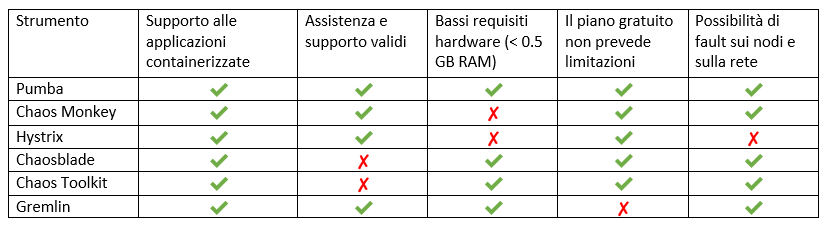
\includegraphics[width=14cm, height=4cm]{images/tabella.png}
            \caption {Pumba presenta tutti i requisiti più importanti}
            \label {tab:pumba}
        \end{center}
        \end{table}
        vista la possibilità di usufruire di una suite completa di interventi in modo gratuito, i requisiti hardware praticamente trascurabili, la distribuzione con licenza Apache 2.0 \cite{Apache} e l'esistenza di un eseguibile scaricabile e usabile direttamente sui nodi che eseguono i container Docker, la scelta finale è stata Pumba. 
        
        Pumba permette di effettuare le seguenti operazioni: 
        \begin{itemize}
            \item \textit{Kill}: consente di terminare un container, specificando il segnale desiderato da inviare al processo nel container.
            
            \item \textit{Pause}: permette di sospendere temporaneamente il processo all'interno del container, specificando la possibilità di riavvio automatico
            
            \item \textit{Netem}: permette di utilizzare gli strumenti di \textit{Traffic Control} (tc) \cite{tc} tramite i comandi:
            \begin{itemize}
                \item \textit{Delay}: aumenta la latenza di tutti i pacchetti in uscita dai container specificati
                \item \textit{Loss}: aggiunge una probabilità (impostabile) di perdita di pacchetti
                \item\textit{ Rate}: limita la banda per tutti i pacchetti in uscita dai container specificati
                \item \textit{Duplicate}: aggiunge una probabilità (impostabile) di duplicazione di pacchetti
                \item \textit{Corrupt}: aggiunge una probabilità (impostabile) di corruzione di pacchetti
            \end{itemize}
            
            \item \textit{Stress}: simula un aumento di utilizzo delle risorse indicate dei container specificati
        \end{itemize}
       Ogni comando possiede una collezione di flag e attributi per specificare la durata, gli intervalli e le modalità di applicazione dei metodi (indicando, ad esempio, l’interfaccia di rete per \textit{netem} o la componente nel caso di stress).\\\\Alcuni esempi di comandi vengono riportati di seguito:\\\\
        \texttt{pumba netem --duration 5m delay --time 3000 mydb} (delay di 3 secondi su tutti i pacchetti in uscita sull’interfaccia default del container mydb)\\\\
        \texttt{pumba netem --duration 5m corrupt --percent 10 mydb} (corruzione del 10\% dei pacchetti in uscita dal container mydb per 5 minuti) \\\\
        \texttt{pumba stress --duration 5m CPU--load10 mydb} (stress della CPU con carico al 10\% del container mydb per 5 minuti)\\\\
        \texttt{pumba --random --interval 1s kill --signal SIGKILL} (invio di SIGINT a container selezionati pseudorandomicamente, con intervallo di un secondo)\\
    
        \subsection{Automazione dei test: FogMonK}
        \label{subsec:FogMonK}
        FogMonK è un programma realizzato in Java, che si pone l’obiettivo di automatizzare l'esecuzione degli esperimenti di Chaos tramite Pumba, monitorare lo stato del sistema e raccogliere i dati di FogMon, senza la necessità di un utente che osservi attivamente il processo.
        
        FogMonK interopera con FogMonEye e, pertanto, sfrutta la creazione di “momenti” (le fasi di un esperimento già descritte in 2.1.4) e sul controllo dei cambiamenti del sistema tra questi ultimi. Più precisamente, FogMonK non si limita a effettuare delle “fotografie” del sistema prima e dopo ogni fase, ma cerca di identificare le cause delle possibili deviazioni.
        
        In base all'esperimento da eseguire, l'utente può specificare un insieme di parametri come input: 
        \begin{itemize}
            \item Tipo di test (\textit{kill, netem, stress}) 
            
            \item Ruolo dei nodi a cui applicare il test (Leader/Follower oppure i nodi specifici, da indicare con il nome del nodo) 
            
            \item Percentuale dei nodi a cui applicare il test, chiaramente non utilizzata qualora vengano indicati i nodi specifici su cui applicare i metodi 
            
            \item Tempo limite per la stabilità 
            
            \item Riavvio automatico in caso di \textit{Node failure} dei nodi 
        \end{itemize}
        Oltre a questi parametri generici troviamo quelli riservati esclusivamente ad alcuni test: 
        \begin{itemize}
            \item In caso di \textit{kill}, il lasso di tempo da attendere tra l’abbattimento di un nodo e quello del successivo 
            
            \item In caso di \textit{netem}, la percentuale di perdita dei pacchetti, la latenza da aggiungere ai nodi o l’utilizzo di banda, in percentuale 
            
            \item In caso di \textit{stress}, la componente da andare a sottoporre a sforzo e la percentuale di utilizzo desiderata 
        \end{itemize}
        La configurazione di input sfrutta un file in formato JSON per ragioni di manutenibilità del codice e facilità nell’implementare nuovi parametri e nuove funzioni.
        
        Per quanto riguarda l'output, FogMonK restituisce le seguenti informazioni al termine di un esperimento: 
        \begin{itemize}
            \item Id di sessione di FogMonEye (ovvero un numero identificativo dell'esperimento)
            
            \item Id dell’esperimento 
            
            \item Sommario dell’input 
            
            \item Elenco dei nodi e delle loro informazioni 
                \begin{itemize}
                \item Nome 
                
                \item Stato prima dell’esperimento (\textit{alive/killed}) 
                
                \item Gruppo di appartenenza iniziale 
                
                \item Ruolo iniziale 
                
                \item Test effettuato 
                
                \item Gruppo di appartenenza finale 
                
                \item Ruolo finale 
                
                \item Stato dopo l’esperimento 
                \end {itemize}
            
            \item Tempo di inizio esperimento (gg/mm/aa, h:m:s:ms) 
            
            \item Tempo di fine esperimento 
            
            \item Tempo di stabilità 
            
            \item Errore sulle misurazioni di latenza e banda 
            
            \item Sommario di verifica delle ipotesi. Questo sommario consiste nell'elenco delle metriche verificate nell'esperimento e nel risultato di tale verifica, pertanto è di fondamentale importanza per comprendere se la seconda stabilità sia stata raggiunta e se le metriche di verifica delle ipotesi rientrino nei valori corretti
            
            \item Superamento del test 
        \end{itemize}
        L'output riesce a rappresentare un momento (inteso come l'insieme degli eventi che vanno dalla stabilità iniziale a quella successiva all'applicazione del metodo), integrando quindi il controllo delle eventuali deviazioni e identificando comportamenti o arresti anomali. Il report di tutti i nodi serve a facilitare l'analisi che l'utente esegue al termine dell'esperimento. Il risultato avrà un aspetto simile alla Figura \ref{fig:output}.
        \begin{figure}
            \begin{center}
                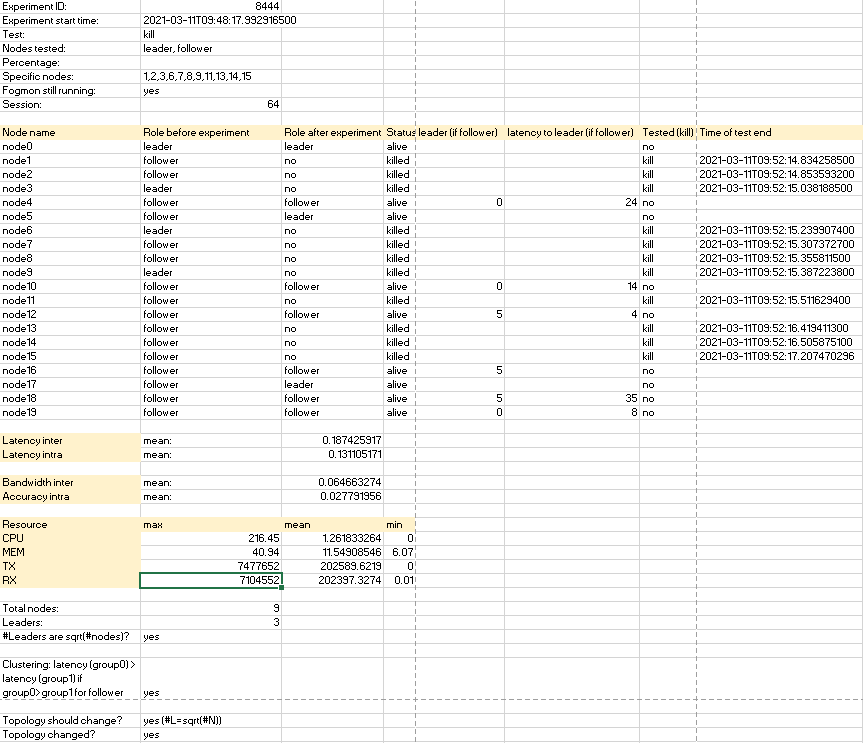
\includegraphics[width=13cm, height=13cm]{images/out.png}
                \caption {Un esempio di output di FogMonK}
                \label{fig:output}
            \end{center}
        \end{figure}

        \paragraph{Fasi di sperimentazione con FogMonK}\mbox{}\newline
        Un esperimento svolto con FogMonK segue l'iter descritto al Capitolo 2.2. Dopo l'avvio del testbed e di FogMon, le fasi sono:
        \begin{itemize}
            \item Verifica della prima stabilità e controllo delle metriche delle \textit{Steady State Hypotesis}. Se le metriche non rientrano nello spettro dei valori accettabili, l'esperimento viene concluso, identificando il problema
            \item Se FogMon raggiunge la prima stabilità, FogMonK sfrutta Pumba per applicare il metodo previsto nella configurazione dell'esperimento
            \item FogMonK attende fino alla validità dell'ipotesi H1 descritta nella Sezione 3.1. Se questa non viene raggiunta, si identifica la deviazione nel report di output
            \item Anche se l'ipotesi H1 viene raggiunta, ma le metriche di H2 e H3 non rientrano nello spettro dei valori accettabili, si rileva una deviazione
            \item Se tutte le \textit{Steady State Hypotesis} sono verificate, l'esperimento termina senza deviazioni identificate
        \end{itemize}
        Ricordiamo che le prime due metriche dell'ipotesi H1 sono:
        \begin{itemize}
            \item L'organizzazione dell'overlay di FogMon in Leader e Follower non cambia per 40 periodi consecutivi di comunicazione Leader-Leader (ovvero 40 volte il valore di \textit{propagation-time}, uno dei parametri di configurazione di FogMon)
            \item Tutte le misurazioni della QoS dei collegamenti e dell'hardware sono state eseguite almeno una volta in ciascun gruppo e mostrano un errore inferiore al 25\%.
        \end{itemize}
        La verifica di H1 sfrutta, per queste prime due metriche, i servizi offerti da FogMonEye. Per tutte le altre verifiche, FogMonK controlla se le metriche descritte nella Sezione 3.1 rientrano nello spettro dei valori accettabili tramite controlli sui file di log dei nodi, interrogazioni ai database e monitoraggio dell'uso delle risorse.
        
        FogMonK invoca comandi Pumba per l'applicazione di tutti i metodi. In particolare:
        \begin{itemize}
            \item Per il metodo \textit{Node failure}, FogMonK lancia l'esecuzione del comando \textit{pumba kill} sui nodi destinati al fallimento
            \item Per il metodo \textit{Link failure}, FogMonK usa il comando \textit{pumba netem} sui nodi collegati dal \textit{link}, specificando l'interfaccia di rete di ciascun nodo
            \item Per il metodo \textit{Stress test}, FogMonK lancia il comando \textit{pumba stress} sui nodi da sottoporre all'esperimento
        \end{itemize}
        I comandi addizionali di Pumba vengono scelti da FogMonK in base alla configurazione di input dell'utente.
        
        \paragraph{Principali classi di FogMonK}
        In Figura \ref{fig:classes} vediamo un diagramma delle classi principali di FogMonK. Di queste, nei successivi paragrafi saranno presentate sinteticamente le tre più importanti per lo svolgimento delle funzioni di FogMonK.
                
        \begin{figure}[H]
            \begin{center}
                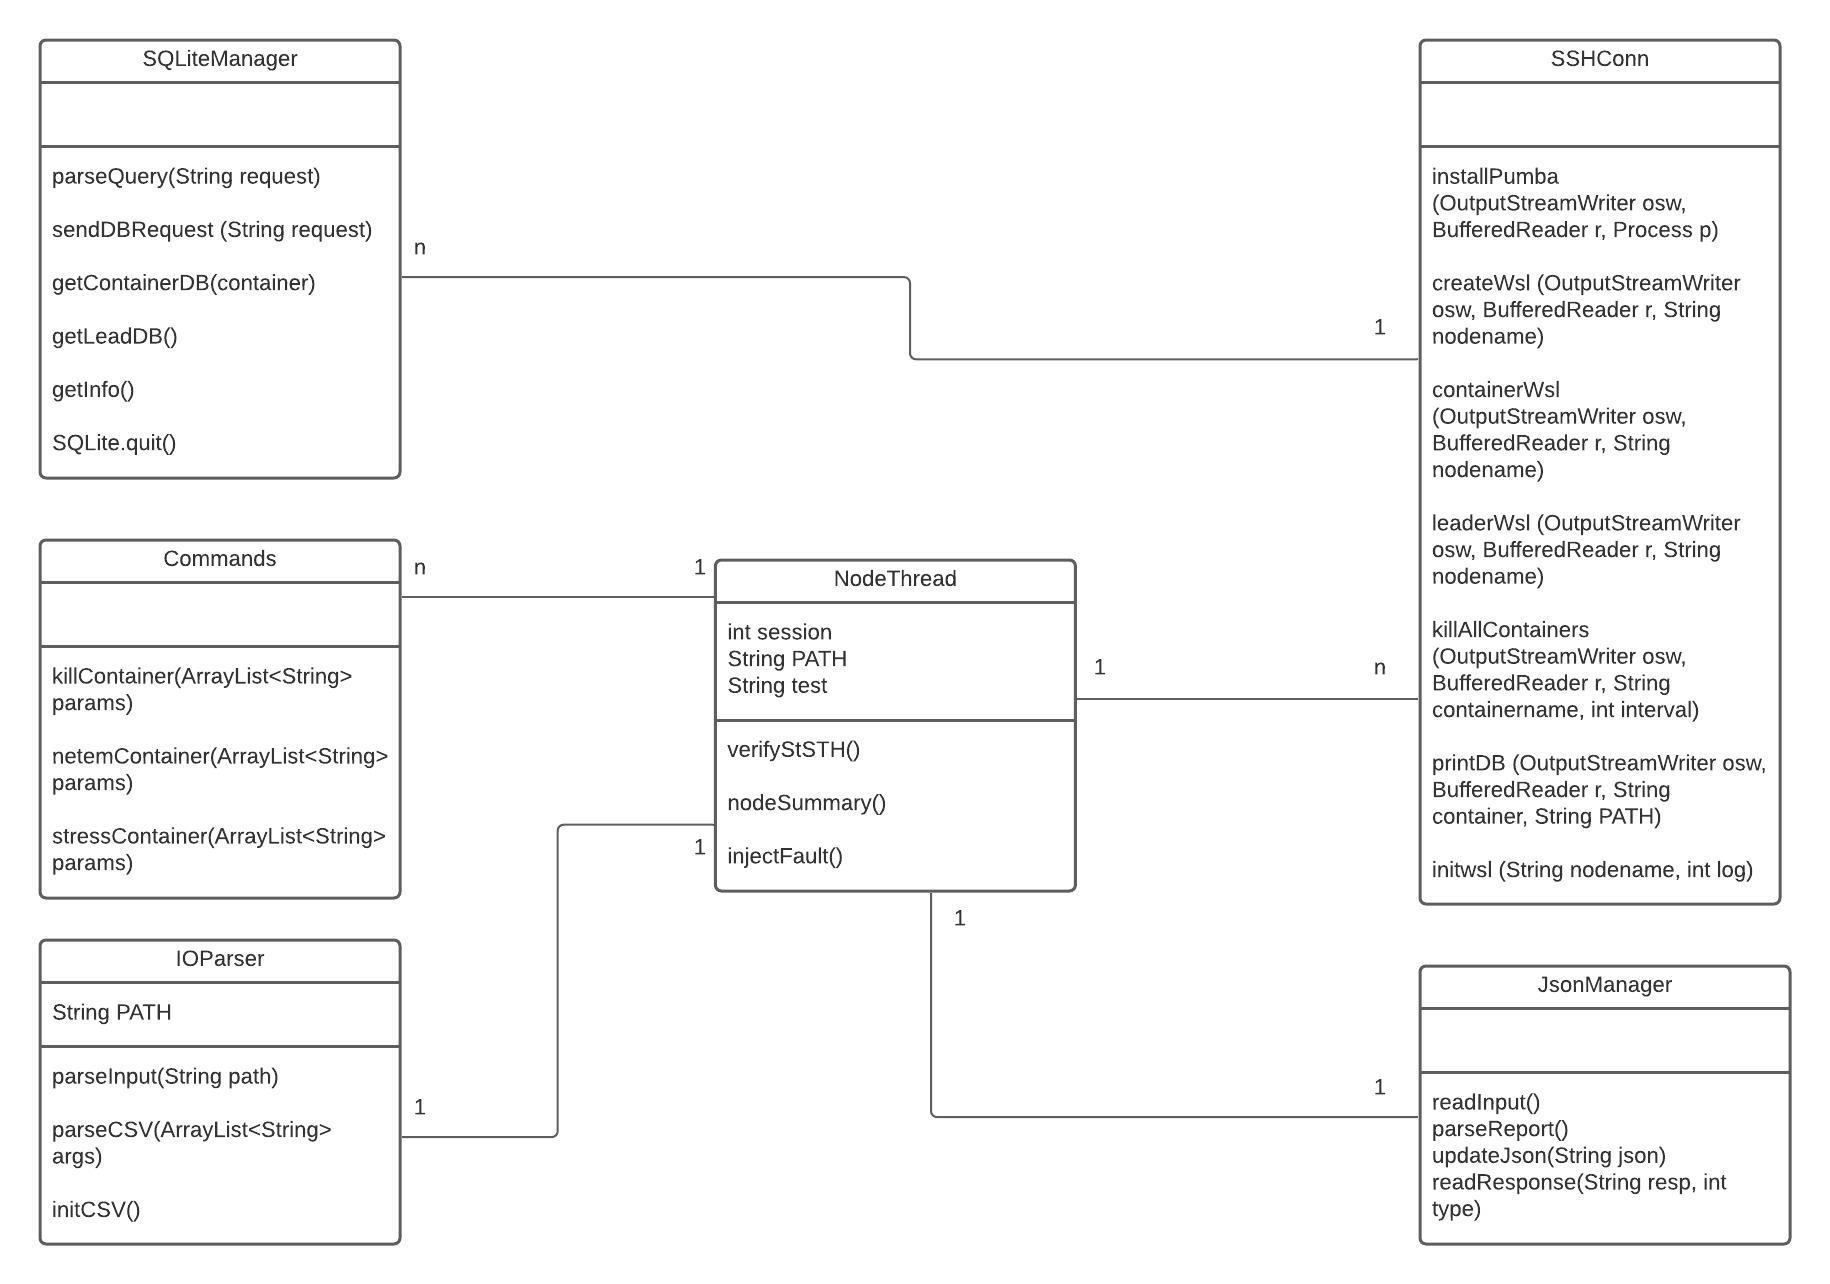
\includegraphics[width=13cm, height=10cm]{images/diag.classi.tesi.jpeg}
                \caption {Organizzazione in classi di FogMonK}
                \label{fig:classes}
            \end{center}
        \end{figure}
        
        \paragraph{La classe JsonManager}\mbox{}\newline
        Come già menzionato, il formato dell’input sfrutta JSON; ne vediamo un esempio nella figura \ref{fig:json}.
        \begin{figure}
            \begin{center}
                \begin{lstlisting}

                    files = ["in"] 
                    name_override = "jsoninput" 
                    data_format = "json" 
                    
                    {
                    "type": "kill", 
                    "nodetype": "leader", 
                    "specnodes": [], 
                    "timelimit": 600, 
                    "percent": 80, 
                    "restartoncrash": "false", 
                    "killtimewait": , 
                    "netemlaten": , 
                    "netemband": , 
                    "stresscomp": 
                    "connum": , 
                    }
                    
                \end{lstlisting}
                \caption {Parametri di input di un esperimento di tipo \textit{Leader failure}}
                \label{fig:json}
            \end{center}
        \end{figure}
        
        Per la raccolta dei dati, la gestione dei dati da scambiare con FogMonEye e, più in generale, per le conversioni di stringhe da e verso JSON, FogMonK contiene la classe JsonParser, di cui riportiamo i metodi più usati e importanti:
        \begin{itemize}
            \item \texttt{readInput()}: si occupa di leggere i dati di ingresso forniti dall'utente nel file JSON. Tali dati verranno poi comunicati al thread principale, incaricato di variare i comandi da lanciare in base ai parametri selezionati
            \item \texttt{parseReport()}: crea una stringa JSON da inviare successivamente a FogMonEye, per aggiornarlo di cambiamenti avvenuti nella topologia di rete (disconnessione di nodi, eliminazione di link, etc)
            \item \texttt{updateJson(String json)}: aggiorna il file di specifica contenente le informazioni sulla rete, viene invocato in caso di connessione/disconnessione di nodi o di creazione/distruzione di link
            \item \texttt{readResponse(String resp, int type)}: converte i dati ottenuti dalle risposte di FogMonEye. Il parametro type indica di che tipo di risposta si tratti (richiesta dei dati di \textit{accuracy} e \textit{performance}, richiesta di \textit{footprint}, conferma della creazione del momento, etc)
        \end{itemize}
        Per evitare di creare un gestore JSON personalizzato, si fa uso delle librerie Google Gson \cite{gson} che semplificano il processo di conversione da \textit{Json Object} a stringa, ma si rivelano molto comode anche nel processo inverso, a patto di avere una classe pronta a incapsulare i dati contenuti nella stringa JSON.
        
        Anche i file contenenti le informazioni sulla topologia e sulle condizioni dei singoli nodi (\textit{spec}) sfruttano la notazione JSON e, con essi, anche i report da inviare a FogMonEye (contenenti le informazioni sulle variazioni della topologia di rete monitorata da FogMon); l’elaborazione di questi file, al crescere del numero di nodi, mostra dei limiti in fatto di efficienza. In futuro, se la dimensione dei dati dovesse aumentare, andrebbe considerata la possibilità di variarne la modalità di rappresentazione in favore di una più efficiente e veloce(YAML XML).
        \paragraph{La classe SSHConn}\mbox{}\newline
        Per il monitoraggio e l'applicazione dei metodi in FogMon, l'installazione di Pumba e la verifica delle ipotesi FogMonK si connette direttamente ai nodi su cui FogMon è distribuito.
        
        Vista la possibilità che Fed4Fire offre di connettersi in SSH ai nodi degli esperimenti istanziati sui loro \textit{testbed}, la soluzione adottata è proprio la creazione di Thread che si occupino di instaurare una connessione con il nodo e di riportare fedelmente ogni dettaglio dell’interazione su dei log dedicati.
        
        Anziché sfruttare librerie di terze parti per le connessioni SSH, FogMonK genera dei terminali usando le chiavi e gli id RSA memorizzati tramite gli strumenti forniti da Jfed; pertanto, per instaurare una connessione è sufficiente lanciare un terminale con il comando “ssh -F ssh-config -I id\_rsa [user]@[nodename]” e specificare un OutputStreamWriter e un InputStreamReader per la comunicazione tra FogMonK e il terminale appena creato.
        
        Per ogni nodo, come menzionato, possono essere instaurate più connessioni, in dettaglio: 
        \begin{itemize}
            \item Una per il monitoraggio del database: 
            FogMonK deve poter controllare i dati del database di ogni nodo per verificarne l’integrità 
            
            \item Una per il monitoraggio del log di FogMon: 
            FogMonK accede ai log di ogni nodo per verificare i possibili errori nella comunicazione tra FogMon e FogMonEye, i \textit{node failure} inattesi, la valutazione che FogMon stesso effettua della qualità del servizio (se insoddisfacente può portare a una riconfigurazione) e la frequenza delle rilevazioni sulla latenza e sulla banda 
            
            \item Una per il lancio di comandi e la raccolta delle risposte: 
            ogni comando, compresi quelli per l'applicazione dei metodi, ha bisogno di un terminale dedicato per la raccolta e l’analisi delle risposte 
             
            \item Una al primo avvio dell’esperimento, per installare Pumba in caso non sia già presente sulla macchina: 
            FogMonK verifica la presenza di Pumba tramite una ricerca nella cartella di installazione predefinita; se assente, lo installa.
        \end{itemize}
        Ogni volta che FogMonK necessita di una connessione, la crea tramite la classe SSHConn. Tutte le connessioni vengono terminate quando esauriscono il loro ruolo, per evitare di dover gestire troppi stream di input e output e rallentare l'esecuzione di FogMonK.
        \paragraph{La classe SQLiteManager}\mbox{}\newline
        La classe SQLiteManager si occupa di incapsulare comandi SQLite3 per i terminali che realizzano le connessioni, di interpretare le risposte delle interrogazioni ai \textit{DataBase} di FogMon e di decapsularle per convertirle in dati utili a FogMonK.
        
        Trattandosi di un accesso ``esterno" ai database, SQLiteManager fornisce un metodo di gestione degli errori di lettura del DB, che possono verificarsi nel caso in cui esso sia in uso da FogMon al momento dell'accesso da parte di FogMonK. In tal caso, FogMonK ripeterà l'interrogazione dopo un intervallo prestabilito. Tra i metodi principali troviamo:
        \begin{itemize}
            \item \texttt{parseQuery(String request)}: esegue la query richiesta in un database precedentemente aperto e salva la risposta nella cartella predefinita
            \item \texttt{sendDBRequest (String request)}: richiede l'accesso a un database per poterlo utilizzare
            \item \texttt{getContainerDB(String container)}: dopo aver richiesto l'accesso, apre il database per accedere ai dati con query
            \item \texttt{getLeadDB()}: apre il database dei nodi leader in cui è invocato
            \item \texttt{getInfo(String op)}: stampa le informazioni richieste in base al parametro \textit{op} con cui è invocato
            \item \texttt {SQLite.quit()}: chiude il database in uso e la console SQLite3 che era aperta nel terminale
        \end{itemize}












\chapter{Esperimenti e Risultati}
In questo capitolo sono descritte le attività di Chaos Testing eseguite nell'ambito dell'esperimento Liscio. Tali attività mirano a trovare delle possibili deviazioni nel comportamento di FogMon tramite l'iniezione volontaria di fallimenti, per identificare le cause di tali deviazioni e mettere a punto FogMon sulla base di quanto scoperto. La sperimentazione ha sfruttato le risorse della federazione dei testbed offerta dal progetto Fed4Fire+, in particolare le risorse dei testbed descritti nella Sezione 3.3: Virtual Wall e CityLab. Per le caratteristiche dei nodi utilizzati, consultare \cite{pcgen2} e \cite{clnodes}.

La sperimentazione è stata condotta nei giorni tra il 9 Marzo e il 3 Aprile, per un totale di 127 esperimenti. Di questi, saranno riportati solo quelli significativi per la scoperta di deviazioni. Tra i test svolti dopo la messa a punto di FogMon, sono esposti gli ultimi 10 per ogni metodo e topologia, per mostrare l'affidabilità e stabilità raggiunte dal prototipo.

Nella Sezione 4.1 sono presentati gli esperimenti che hanno condotto alla scoperta degli errori di Fogmon, trovati mediante le tecniche ispirate al \textit{Chaos Testing}. Questi risultati hanno condotto a una messa a punto di FogMon, che ora è in grado di superare gli stessi test. Di questi test vediamo i risultati nella Sezione 4.2.


Tutti i risultati saranno presentati esplicitando come prima cosa il test effettuato (i.e. \textit{Node Failure}, \textit{Link Failure} o \textit{Stress test}). Gli esperimenti, eseguiti mediante l'uso di FogMonK, seguono la stessa modalità:
\begin{itemize}
    \item Prima verifica delle ipotesi
    \item Applicazione del Metodo
    \item Seconda verifica delle ipotesi
    \item Analisi dei risultati
\end{itemize}
Le tabelle presenti nelle prossime sezioni mostrano i dati di FogMonEye (misurazioni hardware di CPU e Memoria, tempo di stabilità, errore sulle misurazioni della QoS di rete) in determinati scenari. Il valore di \textit{Time to stability} indica il tempo necessario al raggiungimento delle condizioni di validità dell'ipotesi H1 in secondi. I valori di banda e latenza sono espressi in termini di errore percentuale inter-gruppo e intra-gruppo.
    \section{Errori rilevati}
    Di seguito si riportano i risultati più significativi nell'identificazione degli errori di FogMon. Al formato appena menzionato, saranno aggiunte informazioni utili a descrivere il contesto della deviazione:
    \begin{itemize}
        \item Ambiente operativo: topologia, raggiungimento della stabilità.
        \item Evento osservato: reazione da parte di FogMon all'iniezione dei fault
        \item Ipotesi violata (motivo per cui l'evento osservato viene considerato un errore)
        \item Dati di FogMonEye fino alla prima stabilità
    \end{itemize}
        \subsection{Disconnessione inattesa dei leader}
        Il metodo che ha evidenziato questa deviazione è il \textit{Node failure}, in particolare \textit{Leader failure} applicato a un solo Leader scelto in modo pseudocasuale su una rete di 20 nodi. Tutti i nodi sfruttati sono nodi di Virtual Wall \cite{pcgen2}, che hanno 2 CPU quad core da 2,2 GHz e 4 GB di RAM.
        
        Al raggiungimento della prima stabilità (rispetto di H1, H2 e H3, come descritto nella Sezione 3.1) FogMon presentava i dati esposti nelle tabelle \ref{tab:leadercrash} e \ref{tab:leadercrashqos}.
        
        \begin{table}[H]
            \begin{center}
            \caption{Dati di CPU, Memoria e \textit{Time to stability} alla prima stabilità}
            \label{tab:leadercrash}
                \begin{tabular}{|c|c|c|c|c|c|c|c|}
                    \hline
                    Situazione & \textit{Time to stability} & CPU & Memoria\\
                    \hline
                    Init & 292.2 s & 1.78\% & 11.90 MB\\
                    \hline
                \end{tabular}
            \end{center}
        \end{table}
        
        \begin{table}[H]
            \begin{center}
            \caption{Errore sulle misurazioni di banda e latenza alla prima stabilità}
            \label{tab:leadercrashqos}
                \begin{tabular}{|c|c|c|c|c|c|c|c|}
                    \hline
                    Situazione & Latenza intra & Banda intra & Latenza inter & Banda inter\\
                    \hline
                    Init & 13\% &  15\%  &  22\% &  24\%\\
                    \hline
                \end{tabular}
            \end{center}
        \end{table}
        
        Il \textit{Leader failure} ha causato un errore durante la comunicazione tra il nodo terminato e un altro leader, portando alla disconnessione inattesa di quest'ultimo. La seconda verifica delle ipotesi evidenzia dunque una deviazione nel numero di nodi presenti dopo la riconfigurazione di FogMon.
        
        La correzione dell'errore consiste nella modifica dei controlli sulle comunicazioni tra Leader, in modo da evitare la terminazione di FogMon su un nodo qualora questo stia comunicando con un altro nodo soggetto a un fallimento.
        %\subsection{Errore nella configurazione iniziale di FogMon}
        %La distribuzione iniziale di FogMon sul testbed avviene tramite la connessione di un nodo leader e dei restanti nodi follower, che si collegano provvisoriamente al primo leader (in attesa della prima riconfigurazione, volta a eleggere nuovi leader).
        
        
       % Durante la fase preliminare di un \textit{node failure} test sui follower, il leader iniziale ha avviato il processo di ricalcolo, generando un numero casuale; questo, tuttavia, non era un intero positivo (nello specifico log(0)). Tale errore ha causato la disconnessione del leader e, di conseguenza, FogMon ha cessato la sua attività di monitoraggio in quanto privo di leader e incapace di riconfigurarsi.
        
        %L'ipotesi violata è quindi la prima. Nel caso in questione, infatti, dopo 20 minuti dall'avvio FogMon non aveva ancora comunicato con FogMonEye e non aveva effettuato riconfigurazioni, in quanto privo di leader.
        \subsection{Divisione dei gruppi}
        Il metodo utilizzato è il \textit{Node failure}, in particolare quattro \textit{Leader failure} e quattro \textit{Follower failure} per un totale di 8 nodi su una rete di 40. Di questi 40 nodi, 30 sono di forniti da Virtual Wall (con le stesse specifiche già menzionate), e 10 sono nodi di CityLab \cite{clnodes}, che hanno CPU quad core da 1 GHz e 4 GB di RAM.
        
        Al raggiungimento della prima stabilità FogMon presentava i dati esposti nelle tabelle  \ref{tab:groupsplit} e \ref{tab:groupsplitqos}.
        
        \begin{table}[H]
            \begin{center}
                \caption{Dati di CPU, Memoria e \textit{Time to stability} alla prima stabilità}
                \label{tab:groupsplit}
                \begin{tabular}{|c|c|c|c|c|c|c|c|}
                    \hline
                    Situazione & \textit{Time to stability} & CPU & Memoria\\
                    \hline
                    Init & 293.6 s & 2.33\% & 24.70 MB\\
                    \hline
                \end{tabular}
            \end{center}
        \end{table}
        
        \begin{table}[H]
            \begin{center}
            \caption{Errore sulle misurazioni di banda e latenza alla prima stabilità}
                \label{tab:groupsplitqos}
                \begin{tabular}{|c|c|c|c|c|c|c|c|}
                    \hline
                    Situazione & Latenza intra & Banda intra & Latenza inter & Banda inter\\
                    \hline
                    Init & 11\% &  12\%  &  25\% &  23\%\\
                    \hline
                \end{tabular}
            \end{center}
        \end{table}
        
        L'applicazione del metodo di \textit{Node failure} ha innescato il ricalcolo della topologia, ma la comunicazione tra due leader e il resto della rete si è interrotta; FogMonEye non era in grado di definire una stabilità perchè riceveva dati da due reti ormai separate. La seconda verifica delle ipotesi mette in luce la violazione di H1.
        
        L'errore era causato da un problema di sincronizzazione degli accessi al database condiviso dai leader: troppi accessi paralleli, infatti, causavano il blocco di un thread responsabile della propagazione di alcuni dati tra i leader stessi, portando infine alla separazione dei gruppi. 
        
        La deviazione ha permesso di identificare e correggere il bug tramite l'ottimizzazione degli accessi al database.
        \subsection{Riconfigurazione ciclica}
        Il metodo che ha evidenziato questa deviazione è il \textit{Link failure}, applicato a un nodo su una rete di 20.
        
        Al raggiungimento della prima stabilità (e quindi verificate le ipotesi H1, H2 e H3 descritte in 3.1), FogMon presentava i dati esposti nelle tabelle \ref{tab:reconfig} e \ref{tab:reconfigqos}.
        
        \begin{table}[H]
            \begin{center}
            \caption{Dati di CPU, Memoria e \textit{Time to stability} alla prima stabilità}
            \label{tab:reconfig}
                \begin{tabular}{|c|c|c|c|c|c|c|c|}
                    \hline
                    Situazione & \textit{Time to stability} & CPU & Memoria\\
                    \hline
                    Init & 280.0 s & 0.95\% & 40.22 MB\\
                    \hline
                \end{tabular}
            \end{center}
        \end{table}
        
        \begin{table}[H]
            \begin{center}
            \caption{Errore sulle misurazioni di banda e latenza alla prima stabilità}
            \label{tab:reconfigqos}
                \begin{tabular}{|c|c|c|c|c|c|c|c|}
                    \hline
                    Situazione & Latenza intra & Banda intra & Latenza inter & Banda inter\\
                    \hline
                    Init & 8\% &  9\%  &  20\% &  18\%\\
                    \hline
                \end{tabular}
            \end{center}
        \end{table}
        
        L'applicazione del metodo di \textit{Link failure} ha interrotto la comunicazione del nodo (Leader). FogMon ha rilevato un peggioramento della qualità del \textit{clustering} tramite l'indice di qualità, innescando la riconfigurazione dell'overlay di monitoraggio. Gli indici calcolati successivamente non hanno mai rispettato la soglia, causando riconfigurazioni cicliche che hanno impedito il rispetto dell'ipotesi H1.
        
        La modifica consiste nella messa a punto del sistema di calcolo dell'indice di qualità e nell'innalzamento della soglia limite di tale indice, per evitare che il ricalcolo venga innescato nuovamente prima di raggiungere la stabilità definita da H1.
    \newpage   
    \section{Risultati dopo le correzioni}
    Riportiamo i risultati degli esperimenti dopo le correzioni menzionate nei paragrafi precedenti; sarà presentata una media dei valori del sistema a stabilità iniziale e, in seguito, la stessa media calcolata  dopo la seconda stabilità (raggiunta dopo l'iniezione dei fallimenti e l'eventuale riconfigurazione di FogMon). Come accennato in (4.1), i valori riportati sono quelli indicati da FogMonEye.
    
    I Metodi esposti sono quelli indicati nella Sezione 3.1, per maggiori dettagli su tutti gli esperimenti si veda l'appendice (\ref{AppA}).
        \subsection{Metodo \textit{Node failure}}
        Per ogni batteria da 10 esperimenti, sono stati effettuati i test esposti in Tabella \ref{tab:nodefail}. Nella consultazione, si noti che:
        \begin{itemize}
            \item I \textit{Follower failure} (FF) rappresentano 4 dei 10 test per ogni topologia, e prevedono il fallimento di 1, 2, 4 e 4 Follower rispettivamente,
            \item I \textit{Leader failure} (LF) rappresentano 4 dei 10 test per ogni topologia, e prevedono il fallimento di 1, 2, 3 e 3 leader rispettivamente,
            \item I \textit{Leader-Follower failure} (LFF) rappresentano 2 dei 10 test per ogni topologia, e prevedono il fallimento di 4 Leader e 4 Follower in ogni 'esperimento.
        \end{itemize}
        Questi esperimenti saranno raggruppati sotto il nome di \textit{Node failure}, dato che consistono tutti nel fallimento di uno o più nodi.
        
         Nelle tabelle \ref{tab:nodefail20}, \ref{tab:nodefail30} e \ref{tab:nodefail40}  sono descritti i valori della stabilità iniziale (prima verifica di H1, H2 e H3), riportati come \textit{init} e quelli della seconda stabilità (ovvero la seconda verifica di H1, H2 e H3) dopo l'applicazione del metodo \textit{Node failure} per quanto riguarda i valori di CPU, Memoria e \textit{Time to stability}. Analogamente, le tabelle \ref{tab:nodefail20qos}, \ref{tab:nodefail30qos} e \ref{tab:nodefail40qos} indicano gli errori delle rilevazioni sulla QoS di rete (banda e latenza). 
        
        Tutte le tabelle appena menzionate sono esposte a gruppi di due, e indicano rispettivamente le medie dei risultati degli esperimenti su topologie da 20, 30 e 40 nodi. I valori esposti si riferiscono agli ultimi 10 esperimenti effettuati su ogni topologia.
        \newpage
        
        \begin{table}[H]
            \caption{Organizzazione degli esperimenti di \textit{Node failure}}
            \label{tab:nodefail}
            \begin{center}
                \begin{tabular}{|c|c|c|c|c|c|c|c|}
                      \hline
                    Numero di nodi & Test & Numero di test\\
                    \hline
                    20 & FF & 4 \\
 
                    20 & LF & 4 \\

                    20 & LFF & 2 \\
                    \hline
                    30 & FF & 4 \\

                    30 & LF & 4 \\

                    30 & LFF & 2 \\
                    \hline
                    40 & FF & 4 \\

                    40 & LF & 4 \\

                    40 & LFF & 2 \\
                    \hline
                \end{tabular}
            \end{center}
        \end{table}
        
        \begin{table}[H]
            \caption{Dati di CPU, Memoria e \textit{Time to stability} di \textit{Node failure} su 20 nodi}
            \label{tab:nodefail20}
            \begin{center}
                \begin{tabular}{|c|c|c|c|c|c|c|c|}
                      \hline
                    Situazione & \textit{Time to stability} & CPU & Memoria\\
                    \hline
                    Init & 301.6 s & 2.12\% & 41.2 MB\\
                    \hline
                    Final & 291.3 s  & 3.0\% & 38.3 MB\\
                    \hline
                \end{tabular}
            \end{center}
        \end{table}
        
        \begin{table}[H]
            \caption{Risultati degli errori di misurazione di banda e latenza degli esperimenti di \textit{Node failure} su 20 nodi}
            \label{tab:nodefail20qos}
            \begin{center}
                \begin{tabular}{|c|c|c|c|c|c|c|c|}
                    \hline
                    Situazione & Latenza intra & Banda intra & Latenza inter & Banda inter\\
                    \hline
                    Init & 8\% &  3\%  & 11\% &  10\%\\
                    \hline
                    Final & 7\% &  6\%  &  12\% &  14\%\\
                    \hline
                \end{tabular}
            \end{center}
        \end{table}
        
        \begin{table}[H]
            \caption{Dati di CPU, Memoria e \textit{Time to stability} di \textit{Node failure} su 30 nodi}
            \label{tab:nodefail30}
            \begin{center}
                \begin{tabular}{|c|c|c|c|c|c|c|c|}
                     \hline
                    Situazione & \textit{Time to stability} & CPU & Memoria\\
                    \hline
                    Init & 270.1 s & 3.1\% & 39.2 MB\\
                    \hline
                    Final & 299.2 s  & 3.2\% & 36.2 MB\\
                    \hline
                \end{tabular}
            \end{center}
        \end{table}
        
        \begin{table}[H]
            \caption{Risultati degli errori di misurazione di banda e latenza degli esperimenti di \textit{Node failure} su 30 nodi}
            \label{tab:nodefail30qos}
            \begin{center}
                \begin{tabular}{|c|c|c|c|c|c|c|c|}
                    \hline
                    Situazione & Latenza intra & Banda intra & Latenza inter & Banda inter\\
                    \hline
                    Init & 4\% &  9\%  & 12\% &  15\%\\
                    \hline
                    Final & 7\% &  4\%  &  11\% &  15\%\\
                    \hline
                \end{tabular}
            \end{center}
        \end{table}
        
        \begin{table}[H]
            \caption{Dati di CPU, Memoria e \textit{Time to stability} di \textit{Node failure} su 40 nodi}
            \label{tab:nodefail40}
            \begin{center}
                \begin{tabular}{|c|c|c|c|c|c|c|c|}
                     \hline
                    Situazione & \textit{Time to stability} & CPU & Memoria\\
                    \hline
                    Init & 290.1 s & 0.73\% & 29.3 MB\\
                    \hline
                    Final & 302.6 s  & 1.9\% & 31.1 MB\\
                    \hline
                \end{tabular}
            \end{center}
        \end{table}
        
        \begin{table}[H]
            \caption{Risultati degli errori di misurazione di banda e latenza degli esperimenti di \textit{Node failure} su 40 nodi}
            \label{tab:nodefail40qos}
            \begin{center}
                \begin{tabular}{|c|c|c|c|c|c|c|c|}
                    \hline
                    Situazione & Latenza intra & Banda intra & Latenza inter & Banda inter\\
                    \hline
                    Init & 10\% &  6\%  & 13\% &  12\%\\
                    \hline
                    Final & 8\% &  8\%  &  7\% &  11\%\\
                    \hline
                \end{tabular}
            \end{center}
        \end{table}
        
        Contrariamente a quanto osservato in (4.1), dopo la messa a punto di FogMon tutti i valori indicano un comportamento del prototipo nella norma. La verifica di H1, H2 e H3  effettuata tramite FogMonK, quindi, è sempre andata a buon fine.
        \subsection{Metodo \textit{Link failure}}
        Seguendo lo stesso criterio dei \textit{Node failure}, si riportano in tabella \ref{tab:linkfail} i risultati dei test basati sul metodo di \textit{Link failure} (Sezione 3.1.2), effettuati su topologie da 20 nodi. Di questi, 10 sfruttano i nodi offerti da Virtual Wall e 10 quelli offerti da CityLab. L'esperimento prevede la riduzione della banda disponibile su un \textit{link} fino a portarla a 0.1 Mb/s, indipendentemente dal suo valore originario, e l'aumento della latenza a 500 ms per i primi 5 esperimenti, e la stessa operazione su 2 \textit{link} selezionati randomicamente per gli altri 5.
        
        \begin{table}[H]
            \caption{Dati di CPU, Memoria e \textit{Time to stability} di \textit{Link failure}}
            \label{tab:linkfail}
            \begin{center}
                \begin{tabular}{|c|c|c|c|c|c|c|c|}
                     \hline
                    Situazione & \textit{Time to stability} & CPU & Memoria\\
                    \hline
                    Init & 224.8 s & 1.7 \% & 20.1 MB\\
                    \hline
                    Final & 269.0 s & 1.8\% & 22.4 MB\\
                    \hline
                \end{tabular}
            \end{center}
        \end{table}
        
        \begin{table}[H]
            \caption{Risultati degli errori di misurazione di banda e latenza degli esperimenti di \textit{Link failure} su 20 nodi}
            \label{tab:linkfail20qos}
            \begin{center}
                \begin{tabular}{|c|c|c|c|c|c|c|c|}
                    \hline
                    Situazione & Latenza intra & Banda intra & Latenza inter & Banda inter\\
                    \hline
                    Init & 6\% &  2\%  & 9\% &  12\%\\
                    \hline
                    Final & 5\% &  7\%  &  6\% &  18\%\\
                    \hline
                \end{tabular}
            \end{center}
        \end{table}
        
       L'unico cambiamento osservabile è l'aumento dell'errore delle misurazioni di banda e latenza inter-gruppo, rispetto alla condizione iniziale, del 6\%. Si tratta tuttavia di un aumento minimo, che rientra ampiamente nello spettro dei valori accettabili e, pertanto, non può considerarsi una deviazione.
        \subsection{Metodo \textit{Stress Test}}
       Infine, sempre seguendo il criterio visto per \textit{Node failure} e \textit{Link failure}, si riportano nelle tabelle  \ref{tab:stresstest}  e  \ref{tab:stresstestqos}  i risultati del'applicazione del metodo \textit{Stress test}. Gli esperimenti sono stati condotti su topologie da 20 nodi, tutti distribuiti su Virtual Wall, e prevedono la simulazione dell'uso di 7 core sugli 8 disponibili e di 500 MB di RAM.
        
        \begin{table}[H]
            \caption{Dati di CPU, Memoria e \textit{Time to stability} degli esperimenti di \textit{Stress Test}}
            \label{tab:stresstest}
            \begin{center}
                \begin{tabular}{|c|c|c|c|c|c|c|c|}
                     \hline
                    Situazione & \textit{Time to stability} & CPU & Memoria\\
                    \hline
                    Init & 299.8 s & 1.3\% & 40.0 MB\\
                    \hline
                    Final & 289.7 s  & 713.7\% & 530.2 MB\\
                    \hline
                \end{tabular}
            \end{center}
        \end{table}
        
        \begin{table}[H]
            \caption{Risultati degli errori di misurazione di banda e latenza degli esperimenti di \textit{Stress Test}}
            \label{tab:stresstestqos}
            \begin{center}
                \begin{tabular}{|c|c|c|c|c|c|c|c|}
                    \hline
                    Situazione & Latenza intra & Banda intra & Latenza inter & Banda inter\\
                    \hline
                    Init & 4\% &  3\%  &  9\% &  8\%\\
                    \hline
                    Final & 5\% &  5\%  &  3\% &  10\%\\
                    \hline
                \end{tabular}
            \end{center}
        \end{table}
        Si noti che il valore della CPU oltre il 100\% indica l'uso di più core (200\%, ad esempio, implica l'utilizzo del processore per una potenza pari a quella di 2 core sfruttati al massimo).
        
        Nel valutare i dati esposti, si consideri che l'architettura su cui sono stati svolti gli esperimenti con metodo \textit{Stress test} (pcgen2 \textit{Nodes}\cite{pcgen2}) sfrutta nodi con CPU \textit{2x Quad core Intel E5520 (2.2GHz)}. La percentuale di stress imposta dunque rispecchia quella rilevata dalle misurazioni di FogMon, come confermato dalla verifica delle ipotesi effettuata tramite FogMonK.
        
        Com'è facilmente osservabile, un aumento considerevole di uso della CPU ed uno più modesto dell'uso della RAM non influisce sui tempi per la stabilità nè sull'accuratezza delle misurazioni di banda e latenza.

\chapter{Conclusioni}
In questa tesi, è stata presentata una sperimentazione sull’uso di tecniche ispirate al Chaos Engineering per testare e valutare il comportamento di FogMon, un prototipo di monitoraggio non intrusivo distribuito per reti Fog, in condizioni di turbolenza della rete (es. fallimento di nodi, degradazione della QoS dei collegamenti). Dopo aver riepilogato alcune conoscenze preliminari necessarie (Capitolo 2), è stato descritto il processo di pianificazione e implementazione degli esperimenti (Capitolo 3) e il set di risultati ottenuti (Capitolo 4).
Di seguito saranno descritti questi risultati , per quanto riguarda la progettazione, l'implementazione e l'esito della sperimentazione, oltre a una considerazione sui possibili sviluppi futuri di questo progetto.
    
    \section{Discussione Critica dei Risultati Ottenuti}
    In questa sezione sono descritti gli esiti del lavoro svolto, valutando i vantaggi e gli svantaggi degli esperimenti di \textit{Chaos Engineering} applicati, e l'esito della sperimentazione, per discutere le informazioni ottenute e confrontarle con gli obiettivi iniziali.
        
        \paragraph{Vantaggi della sperimentazione}\mbox{}\\
            
        Gli esperimenti condotti hanno portato alla scoperta di alcune deviazioni nell'esecuzione di FogMon, (come evidenziato nella Sezione 4.1) e, conseguentemente, hanno permesso di correggere tali errori per migliorare la resilienza del prototipo. L'applicazione delle tecniche ispirate al \textit{Chaos Engineering} dunque ha portato al raggiungimento dell'obiettivo iniziale di evidenziare falle in FogMon e di fornire dati utili per metterlo a punto di conseguenza.
        
        Non è possibile escludere a priori che tali errori potessero essere rilevati anche con altre modalità di testing, ma in generale, possiamo intuire come le tecniche di \textit{Chaos Engineering} possano rivelarsi utili nel rinforzare la \textit{fault tolerance} dei sistemi distribuiti. Nel caso peggiore (ossia quando la sperimentazione non dovesse portare alla scoperta di deviazioni), l'investimento necessario a effettuare i test conferma la validità e la resilienza del software e fornisce dati importanti, grazie monitoraggio del suo comportamento; in tutti gli altri scenari, apporta informazioni preziose ad aumentare la resilienza del software testato.
        
        Un altro risultato fondamentale di questo lavoro consiste nel contributo apportato al progetto LiSCIo: la sperimentazione ha permesso di fornire un ampio set di dati di testing. In particolare, nel rapporto conclusivo di LiSCIo \cite{FogMon} si descrive anche la fase di test di FogMon, di cui fanno parte i \textit{Node failure} e i \textit{Link failure} e i cui dati sono in parte derivanti dagli esperimenti condotti per questa tesi. Ad esempio, la fase di testing di FogMon comprende un'area di \textit{soft failure}, ossia di fallimenti più probabili e relativamente poco incisivi sul funzionamento del prototipo, costituita interamente dalle applicazioni dei metodi di \textit{Follower failure} descritte in 3.1.2. e, pertanto, coincidenti con quanto svolto ai fini di questa tesi. 
        
        Altri contributi riguardano il testing di alcune topologie per i metodi \textit{Leader failure} e \textit{Leader-Follower failure}, i cui risultati sono in parte ripresi dalla sperimentazione eseguita con le tecniche ispirate al \textit{Chaos testing}. 
        
        Infine, le fasi preliminari della sperimentazione sui \textit{Link failure} e \textit{Node failure}, descritte nel Capitolo 4, hanno evidenziato alcuni problemi nel calcolo dell'errore della QoS di rete in FogMonEye, tempestivamente corretti e integrati nelle rilevazioni riportate in 4.2.2.
        
        
        \paragraph{Svantaggi della sperimentazione}\mbox{}\\
        
        Il lavoro svolto, tuttavia, incontra alcuni limiti. Ad esempio, le ipotesi descritte nella Sezione 3.1 descrivono buona parte del comportamento di FogMon in condizioni di buon funzionamento, ma la verifica delle operazioni di \textit{gossiping} dei leader richiede maggiore attenzione. 
        In particolare, sarebbe opportuno intensificare il controllo dei dati scambiati tra i Leader per verificare che i loro database presentino le informazioni corrette al termine delle comunicazioni tra gruppi. Questa sperimentazione può essere effettuata andando a definire una quarta ipotesi, che assuma il funzionamento delle appena citate operazioni di \textit{gossiping}. Seguendo poi l'iter descritto al Capitolo 3, dovrebbero essere definite delle metriche per la misurazione della correttezza dei parametri per valutare tale ipotesi. I metodi utilizzati e descritti nella Sezione 3.1.2, intuitivamente, dovrebbero essere in grado di coprire anche gli esperimenti per questa nuova ipotesi.
            
        Inoltre, eseguire più esperimenti contemporaneamente richiede di avviare istanze diverse di FogMonK, che non fornisce nativamente la possibilità di eseguire più test allo stesso momento. I metodi applicati (e i cui risultati sono descritti nella Sezione 4.2) non sono stati parallelizzati, ma il Chaos Engineering incoraggia la sperimentazione di più ``turbolenze" simultanee. Sarebbe interessante, ad esempio, combinare un \textit{Follower failure} con il \textit{Link failure} del Leader di riferimento per testare la velocità di reazione del Leader stesso, oppure integrare lo \textit{Stress Test} con il \textit{Link failure} per verificare la velocità di FogMon nel propagare i peggioramenti delle condizioni dei nodi in condizioni di rete ostili.

    \section{Possibili Sviluppi Futuri}
    Il prosieguo di questa sperimentazione può includere alcune migliorie a FogMonK e al piano di test. In particolare:
    \begin{itemize}
        \item Effettuare un periodo ulteriore di osservazione per includere nel piano degli esperimenti la verifica del \textit{Gossiping}, con la formulazione di un'ipotesi e l'assegnazione delle relative metriche di valutazione e dei metodi.
        \item Integrare il supporto a più esperimenti di Chaos contemporanei in modo da creare condizioni di \textit{Chaos} più complete e simulare fallimenti simultanei, perfezionando il sistema di verifica delle ipotesi per gestire più riconfigurazioni e monitorare l'applicazione di più Metodi
        \item Per la verifica dell'ipotesi \textbf{Tempo massimo di configurazione} (H1), descritta nella Sezione 3.1, sarebbe utile estendere le funzionalità di FogMonK, aumentando il periodo di monitoraggio, fino a includere la fase di riconfigurazione di FogMon che, al momento, è ignorata. Questa intensificazione dei controlli consentirebbe di fornire più dati utili nel caso in cui si dovessero scoprire ulteriori deviazioni (ad esempio, nella verifica di una nuova \textit{Steady state hypotesis} basata sulle operazioni di \textit{gossiping}).
        \item La natura di FogMonK, improntata all'ispezione e al monitoraggio dell'attività di FogMon, rende difficile salire di livello e renderlo uno strumento di Chaos Engineering per tutte le applicazioni distribuite. Per fare ciò, è necessario invece creare un nuovo prototipo incentrato sul \textit{fault management}, ma con delle API che permettano di implementare la verifica delle ipotesi tramite delle metriche personalizzabili. In tal modo, sarebbe possibile fornire uno strumento più completo di quelli attuali (come i software descritti nella Sezione 3.2) che sono unicamente volti al \textit{fault injection} e non si occupano di implementare le fasi successive di un \textit{Chaos Experiment}.
    \end{itemize}
    

\newpage
\printbibliography

\newpage
\appendix
%\chapter{}

%\chapter{}
\newpage

\chapter{}
\label{AppA}
    In tabella \ref{tab:NF20}, \ref{tab:NF30} e \ref{tab:NF40}, vediamo il risultato degli ultimi 10 esperimenti di tipo \textit{Node failure} in termini di rilevazioni di \textit{Time to stability}, CPU e Memoria. Similmente, nelle tabelle \ref{tab:nodefail20qos2}, \ref{tab:nodefail30qos2} e \ref{tab:nodefail40qos2} si riportano i dati sugli errori di misurazione di banda e latenza intergruppo e intragruppo. Gli esperimenti comprendono \textit{Leader failure}, \textit{Follower failure} e una combinazione dei due, come descritto nella Sezione 4.2. Nella consultazione, si tenga presente che la sigla FF indica \textit{Follower failure}, LF indica \textit{Leader failure} e LFF indica \textit{Leader-Follower failure}.
    Gli esperimenti di tipo \textit{Follower failure}, come riscontrabile nelle tabelle, non causano il ricalcolo dell'overlay di FogMon
    \begin{table}[H]
    \caption{Dati di CPU, Memoria e \textit{Time to stability} di \textit{Node failure} su 20 nodi}
    \label{tab:NF20}
    \begin{center}
        \begin{tabular}{|c|c|c|c|c|c|c|c|}
            \hline
            Situazione & \textit{Time to stability} & CPU & Memoria & Ricalcolo\\
            \hline
            Init & 301.6 s & 2.12 \% & 41.2 MB & -\\
            FF    & 308.1 s  & 1.8 \%  & 39.9 MB & No\\
            FF    & 307.6 s  & 3.4 \%  & 41.2  MB & No\\
            FF    & 295.6 s  & 1.2 \%  & 49.3  MB & No\\
            FF    & 300.1 s  & 0.6 \%  & 39.6  MB & No\\
            LF    & 258.5 s  & 3.6 \%  & 38.4  MB & Si\\
            LF    & 312.9 s  & 2.3 \%  & 38.1  MB & Si\\
            LF    & 273.2 s  & 2.7 \%  & 47.3  MB & Si\\
            LF    & 300.1 s  & 2.7 \%  & 35    MB & Si\\
            LFF   & 314.6 s  & 2.3 \%  & 29.1  MB & Si\\
            LFF   & 315.2 s  & 1.6 \%  & 31.9  MB & Si\\
            \hline
        \end{tabular}
        \end{center}
    \end{table}
    
    \begin{table}[H]
    \caption{Risultati degli errori di misurazione di banda e latenza degli esperimenti di \textit{Node failure} su 20 nodi}
    \label{tab:nodefail20qos2}
    \begin{center}
        \begin{tabular}{|c|c|c|c|c|c|c|c|}
            \hline
            Situazione & Latenza intra & Banda intra & Latenza inter & Banda inter\\
            \hline
            Init & 8 \%   & 3 \%   & 11 \%  & 10 \%   \\
            FF    & 5 \%   & 9 \%   & 14 \%  & 16 \%   \\
            FF    & 6 \%   & 3 \%   & 11 \%  & 18 \%   \\
            FF    & 15 \%  & 4 \%   & 16 \%  \%  & 13 \%   \\
            FF    & 10 \%  & 8 \%   & 12 \%  & 18 \%   \\
            LF    & 5 \%   & 6 \%   & 10 \%  & 16 \%   \\
            LF    & 10 \%  & 8 \%   & 10 \%  & 12 \%   \\
            LF    & 3 \%   & 10 \%  & 13 \%  & 14 \%   \\
            LF    & 3 \%   & 5 \%   & 18 \%  & 9 \%    \\
            LFF    & 13 \%  & 6 \%   & 8 \%   & 9 \%    \\
            LFF   & 6 \%   & 11 \%  & 10 \%  & 13 \%   \\
            \hline
        \end{tabular}
        \end{center}
    \end{table}
        
    \begin{table}[H]
    \caption{Dati di CPU, Memoria e \textit{Time to stability} di \textit{Node failure} su 30 nodi}
    \label{tab:NF30}
    \begin{center}
        \begin{tabular}{|c|c|c|c|c|c|c|c|}
            \hline
            Situazione & \textit{Time to stability} & CPU & Memoria & Ricalcolo\\
            \hline
            Init & 270.1 s & 3.1 \% & 39.2 MB & -\\
            FF    & 291.2 s  & 3.4 \%  & 30.5 MB & No\\
            FF    & 321.6 s  & 7.9 \%  & 50.8 MB & No\\
            FF    & 316 s  & 2.8 \%  & 31.8 MB & No\\
            FF    & 341.3 s  & 1.3 \%  & 35.1 MB & No\\
            LF    & 290.2 s  & 3.4 \%  & 31   MB & Si\\
            LF    & 283.2 s  & 2.7 \%  & 44.9 MB & Si\\
            LF    & 295.9 s  & 2.7 \%  & 39.4 MB & Si\\
            LF    & 311.5 s  & 4.9 \%  & 33   MB & Si\\
            LFF    & 309.3 s  & 3.5 \%  & 32.3 MB & Si\\
            LFF   & 266.3 s  & 4.7 \%  & 37.9 MB & Si\\
            \hline
        \end{tabular}
        \end{center}
    \end{table}
    
    \begin{table}[H]
    \caption{Risultati degli errori di misurazione di banda e latenza degli esperimenti di \textit{Node failure} su 30 nodi}
    \label{tab:nodefail30qos2}
    \begin{center}
        \begin{tabular}{|c|c|c|c|c|c|c|c|}
            \hline
            Situazione & Latenza intra & Banda intra & Latenza inter & Banda inter\\
            \hline
            Init & 4 \%   & 9 \%   & 12 \%  & 15 \%  \\
            FF    & 9 \%   & 5 \%   & 14 \%  & 20 \%   \\
            FF    & 4 \%   & 4 \%   & 8 \%   & 17 \%   \\
            FF    & 4 \%   & 5 \%   & 11 \%  & 12 \%   \\
            FF    & 6 \%   & 4 \%   & 9 \%   & 15 \%   \\
            LF    & 6 \%   & 4 \%   & 11 \%  & 17 \%   \\
            LF    & 8 \%   & 2 \%   & 12 \%  & 16 \%   \\
            LF    & 6 \%   & 3 \%   & 16 \%  & 13 \%   \\
            LF    & 7 \%   & 3 \%   & 10 \%  & 14 \%   \\
            LFF    & 10 \%  & 5 \%   & 12 \%  & 17 \%   \\
            LFF   & 6 \%   & 4 \%   & 10 \%  & 17 \%   \\
            \hline
        \end{tabular}
        \end{center}
    \end{table}
    
    \begin{table}[H]
    \caption{Dati di CPU, Memoria e \textit{Time to stability} di \textit{Node failure} su 40 nodi}
    \label{tab:NF40}
    \begin{center}
        \begin{tabular}{|c|c|c|c|c|c|c|c|}
            \hline
            Situazione & \textit{Time to stability} & CPU & Memoria & Ricalcolo\\
            \hline
            Init & 290.1 s & 0.73 \% & 29.3 MB & -\\
            FF    & 295.2 s  & 4.4 \%  & 23.1 MB & No\\
            FF    & 307.8 s  & 0.6 \%  & 32.7 MB & No\\
            FF    & 315.5 s  & 1.4 \%  & 37   MB & No\\
            FF    & 304.4 s  & 2.7 \%  & 35.5 MB & No\\
            LF    & 305 s    & 2.3 \%  & 29.5 MB & Si\\
            LF    & 294.4 s  & 1.7 \%  & 31.7 MB & Si\\
            LF    & 311.1 s  & 3   \%  & 33.6 MB & Si\\
            LF    & 307.8 s  & 3.1  \% & 38.6 MB & Si\\
            LFF    & 315.2 s  & 2   \%  & 32.9 MB & Si\\
            LFF   & 307.5 s  & 1.2 \%  & 30.9 MB & Si\\
            \hline
        \end{tabular}
        \end{center}
    \end{table}
    
    \begin{table}[H]
    \caption{Risultati degli errori di misurazione di banda e latenza degli esperimenti di \textit{Node failure} su 40 nodi}
    \label{tab:nodefail40qos2}
    \begin{center}
        \begin{tabular}{|c|c|c|c|c|c|c|c|}
            \hline
            Situazione & Latenza intra & Banda intra & Latenza inter & Banda inter\\
            \hline
            Init & 10 \%  & 6 \%   & 13 \%  & 12 \%   \\
            FF    & 14 \%  & 9 \%   & 8 \%   & 11 \%   \\
            FF    & 5 \%   & 7 \%   & 7 \%   & 12 \%   \\
            FF    & 10 \%  & 6 \%   & 5 \%   & 12 \%   \\
            FF    & 10 \%  & 7 \%   & 6 \%   & 12 \%   \\
            LF    & 7 \%   & 6 \%   & 8 \%   & 10 \%   \\
            LF    & 11 \%  & 7 \%   & 6 \%   & 12 \%   \\
            LF    & 7 \%   & 10 \%  & 4 \%   & 6 \%    \\
            LF    & 9 \%   & 7 \%   & 7 \%   & 8 \%    \\
            LFF    & 7 \%   & 9 \%   & 5 \%   & 10 \%   \\
            LFF   & 7 \%   & 8 \%   & 6 \%   & 7 \%    \\
            \hline
        \end{tabular}
        \end{center}
    \end{table}
        
        
        Nelle tabelle \ref{tab:LF20} e \ref{tab:linkfail20qos2} vediamo il risultato degli ultimi 10 esperimenti di tipo \textit{Link Failure}.
        
        
        
    \begin{table}[H]
    \caption{Dati di CPU, Memoria e \textit{Time to stability} di \textit{Link failure} su 20 nodi}
    \label{tab:LF20}
    \begin{center}
        \begin{tabular}{|c|c|c|c|c|c|c|c|}
            \hline
            Situazione & \textit{Time to stability} & CPU & Memoria\\
            \hline
            Init & 224.8 s & 1.7 \% & 20.1 MB\\
            1    & 249.8 s  & 0.8  \% & 15.7 MB\\
            2    & 257.7 s  & 1.6  \% & 23.8 MB\\
            3    & 278.5 s  & 0.5 \%  & 23.3 MB\\
            4    & 266.7 s  & 3   \%  & 19.2 MB\\
            5    & 282.9 s  & 1.3 \%  & 16.9 MB\\
            6    & 289.1 s  & 0.8 \%  & 24.7 MB\\
            7    & 294.8 s  & 1.4 \%  & 19   MB\\
            8    & 293.8 s  & 4.2 \%  & 28.2 MB\\
            9    & 254.9 s  & 1.1 \%  & 14.4 MB\\
            10   & 262.1 s  & 2.2 \%  & 23   MB\\
            \hline
        \end{tabular}
        \end{center}
    \end{table}
    
    \begin{table}[H]
    \caption{Risultati degli errori di misurazione di banda e latenza degli esperimenti di \textit{Node failure} su 20 nodi}
    \label{tab:linkfail20qos2}
    \begin{center}
        \begin{tabular}{|c|c|c|c|c|c|c|c|}
            \hline
            Situazione & Latenza intra & Banda intra & Latenza inter & Banda inter\\
            \hline
            Init & 6 \%   & 2 \%   & 9 \%   & 12 \%   \\
            1    & 5 \%   & 7 \%   & 6 \%   & 13 \%   \\
            2    & 7 \%   & 13 \%  & 8 \%   & 19 \%   \\
            3    & 2 \%   & 6 \%   & 5 \%   & 18 \%   \\
            4    & 4 \%   & 10 \%  & 4 \%   & 22 \%   \\
            5    & 5 \%   & 10 \%  & 6 \%   & 18 \%   \\
            6    & 4 \%   & 5 \%   & 4 \%   & 20 \%   \\
            7    & 4 \%   & 6 \%   & 3 \%   & 19 \%   \\
            8    & 6 \%   & 9 \%   & 6 \%   & 23 \%   \\
            9    & 6 \%   & 7 \%   & 6 \%   & 21 \%   \\
            10   & 4 \%   & 4 \%   & 9 \%   & 16 \%   \\
            \hline
        \end{tabular}
        \end{center}
    \end{table}
        Nelle tabelle \ref{tab:st20} e \ref{tab:stresstest20qos2} vediamo il risultato degli ultimi 10 esperimenti di tipo \textit{Stress Test}.
    \begin{table}[H]
    \caption{Dati di CPU, Memoria e \textit{Time to stability} di \textit{Stress test} su 20 nodi}
    \label{tab:st20}
    \begin{center}
        \begin{tabular}{|c|c|c|c|c|c|c|c|}
            \hline
            Situazione & \textit{Time to stability} & CPU & Memoria\\
            \hline
            Init & 299.8 s & 1.3\% & 40.0 MB\\
            1    & 283.5 s  & 713.4\% & 510.8 MB\\
            2    & 311.2 s  & 710.3\% & 524.3 MB\\
            3    & 262.7 s  & 715.3\% & 527.1 MB\\
            4    & 267.3 s  & 711.8\% & 506.6 MB\\
            5    & 303.8 s  & 710.9\% & 528.5 MB\\
            6    & 262.5 s  & 728.8\% & 524.8 MB\\
            7    & 297.5 s  & 731.3\% & 512.2 MB\\
            8    & 287.9 s  & 721.1\% & 521.6 MB\\
            9    & 302.7 s  & 706.5\% & 515.5 MB\\
            10   & 270.7 s  & 724.9\% & 539  MB\\
            \hline
        \end{tabular}
        \end{center}
    \end{table}
    
    \begin{table}[H]
    \caption{Risultati degli errori di misurazione di banda e latenza degli esperimenti di \textit{Stress test} su 20 nodi}
    \label{tab:stresstest20qos2}
    \begin{center}
        \begin{tabular}{|c|c|c|c|c|c|c|c|}
            \hline
            Situazione & Latenza intra & Banda intra & Latenza inter & Banda inter\\
            \hline
            Init & 4 \% & 3 \% & 9 \% & 8 \%  \\
            1    & 4 \% & 2 \% & 2 \% & 11 \% \\
            2    & 8 \% & 4 \% & 2 \% & 12 \% \\
            3    & 9 \% & 4 \% & 4 \% & 11 \% \\
            4    & 4 \% & 2 \% & 3 \% & 11 \% \\
            5    & 6 \% & 6 \% & 3 \% & 12 \% \\
            6    & 6 \% & 7 \% & 5 \% & 11 \%  \\
            7    & 2 \% & 6 \% & 4 \% & 8  \% \\
            8    & 12 \% & 8 \% & 4 \% & 8  \% \\
            9    & 4 \% & 8 \% & 3 \%  & 10 \% \\
            10   & 11 \% & 6 \% & 4 \% & 10 \% \\
            \hline
        \end{tabular}
        \end{center}
    \end{table}
\newpage

\end{document}
